\documentclass[11pt,openany]{book}
\raggedbottom

% Load packages
\usepackage[utf8]{inputenc} % for unicode input
\usepackage{microtype}
\usepackage{bm}
\usepackage{enumitem}
\usepackage{geometry} % for page layout
\usepackage{hyperref} % for hyperlinks
\usepackage{tocbibind} % includes the bibliography in the table of contents
\usepackage{amsmath, amsfonts, amssymb, amsthm} % for advanced math formatting
\usepackage{lipsum} % generates filler text
\usepackage{fancyhdr}
\usepackage[table]{xcolor} % for cell coloring
\usepackage{graphicx} % for including images
\usepackage{booktabs} % for professional looking tables
\usepackage[normalem]{ulem} % for underlining
\usepackage[document]{ragged2e} % for text alignment
\usepackage{tikz} % for drawing
\usepackage{algorithm}
\usepackage{algpseudocode}
\usepackage{wrapfig}
\usepackage{circuitikz}
\usepackage{caption}
\usepackage{venndiagram}
\usepackage{multicol}
\usepackage{listings}
\usepackage{adjustbox}
\usepackage{multirow}
\usepackage{media9}



% TikZ libraries
\usetikzlibrary{circuits.logic.US, arrows.meta, positioning, calc, fit, decorations.markings, math}

% Document geometry (page size, margins)
\geometry{a4paper, left=20mm, right=20mm, top=25mm, bottom=30mm}

% Custom page style for centered page numbers
\pagestyle{fancy}
\fancyhf{} % Clear all header and footer fields
\fancyhead[RE]{\leftmark} % Left Even pages - Chapter number and name
\fancyhead[RO]{Notes by Ali EL AZDI} % Right Odd pages - Custom message
\fancyfoot[CE,CO]{\thepage} % Centered page number in the footer for both even and odd pages
\renewcommand{\headrulewidth}{0pt}
\renewcommand{\footrulewidth}{0pt}

% Custom commands
\newcommand*\xor{\oplus}
\newcommand{\minidash}{\text{-}}

% Custom spacing command
\makeatletter
\newcommand{\vspacer}[1]{%
  \ifvmode
    \vskip#1\relax
  \else
    \@bsphack
    \vadjust{\vskip#1\relax}
    \@esphack
  \fi
}
\makeatother

%%%%%%%%%%%%%%%%%%% Verilog CODE STYLING %%%%%%%%%%%%%%%%%%%%%%%%%%%%%
\definecolor{keywordcolor}{rgb}{0.5,0.0,0.33}
\definecolor{backgroundcolor}{rgb}{0.95,0.95,1.0}
\definecolor{commentcolor}{rgb}{0.129,0.384,0.529}
\definecolor{stringcolor}{rgb}{0.16,0.00,1.00}
\definecolor{rulecolor}{rgb}{0.46,0.43,0.5}
\definecolor{codegray}{rgb}{0.5,0.5,0.5}

\lstdefinestyle{verilogstyle}{
  language=Verilog,
  basicstyle=\ttfamily\footnotesize,
  backgroundcolor=\color{backgroundcolor},
  commentstyle=\color{commentcolor}\ttfamily, % Add \ttfamily to ensure comments are in typewriter font
  morecomment=[l][\color{commentcolor}\ttfamily]{//}, % Line comment in Verilog
  morecomment=[s][\color{commentcolor}\ttfamily]{/*}{*/}, % Block comments in Verilog
  morekeywords={module, input, output, wire, endmodule, endcase, default, tri, assign, always, if, else, begin, end, case, endcase, parameter}, % Add Verilog keywords
  keywordstyle=\color{keywordcolor},
  stringstyle=\color{stringcolor},
  showstringspaces=false,
  frame=single,
  rulecolor=\color{rulecolor}, % Frame color
  breaklines=true,
  numbers=left,
  numberstyle=\tiny\color{codegray},
  tabsize=2
}

\lstnewenvironment{verilog}
  {\lstset{style=verilogstyle}}
  {}

%%%%%%%%%%%%%%%%%%% C CODE STYLING %%%%%%%%%%%%%%%%%%%%%%%%%%%%%
\definecolor{ckeywordcolor}{rgb}{0.8,0.1,0.1}
\definecolor{cbackgroundcolor}{rgb}{0.95,0.95,0.95}
\definecolor{ccommentcolor}{rgb}{0.0,0.5,0.0}
\definecolor{cstringcolor}{rgb}{0.1,0.1,0.8}
\definecolor{crulecolor}{rgb}{0.5,0.5,0.5}
\definecolor{ccodegray}{rgb}{0.6,0.6,0.6}

\lstdefinestyle{cstyle}{
  language=C,
  basicstyle=\ttfamily\footnotesize,
  backgroundcolor=\color{cbackgroundcolor},
  commentstyle=\color{ccommentcolor}\ttfamily,
  keywordstyle=\color{ckeywordcolor},
  stringstyle=\color{cstringcolor},
  showstringspaces=false,
  frame=single,
  rulecolor=\color{crulecolor},
  breaklines=true,
  numbers=left,
  numberstyle=\tiny\color{ccodegray},
  tabsize=2
}

\lstnewenvironment{cc}
  {\lstset{style=cstyle}}
  {}

%%%%%%%%%%%%%%%%%%% Assembly CODE STYLING %%%%%%%%%%%%%%%%%%%%%%%%%%%%%
\definecolor{akeywordcolor}{rgb}{0.0, 0.2, 0.4}
\definecolor{abackgroundcolor}{rgb}{0.98, 0.99, 1.0}
\definecolor{acommentcolor}{rgb}{0.0, 0.4, 0.6}
\definecolor{astringcolor}{rgb}{0.2, 0.4, 0.8}
\definecolor{arulecolor}{rgb}{0.6, 0.7, 0.8}
\definecolor{acodegray}{rgb}{0.3, 0.4, 0.5}

\lstdefinestyle{assembly}{
  language=[x86masm]Assembler,
  basicstyle=\ttfamily\footnotesize,
  backgroundcolor=\color{abackgroundcolor},
  commentstyle=\color{acommentcolor}\ttfamily,
  keywordstyle=\color{akeywordcolor},
  stringstyle=\color{astringcolor},
  showstringspaces=false,
  frame=single,
  rulecolor=\color{arulecolor},
  breaklines=true,
  numbers=left,
  numberstyle=\tiny\color{acodegray},
  tabsize=2,
  morekeywords={li, and, add, addi, srli, bne}
}

\lstnewenvironment{assembly}
  {\lstset{style=assembly}}
  {}

%%%%%%%%%%%%%%%%%%%%%%%%%%%%%%%%%%%%%%%%%%%%%%%%%%%%%%%%
%%%%%%%%%%%%%%%%%%% JAVA CODE STYLING %%%%%%%%%%%%%%%%%%%%%%%%%%%%%
\definecolor{javakeywordcolor}{rgb}{0.0, 0.0, 0.5}
\definecolor{javabackgroundcolor}{rgb}{0.95, 0.95, 0.95}
\definecolor{javacommentcolor}{rgb}{0.0, 0.5, 0.0}
\definecolor{javastringcolor}{rgb}{0.6, 0.0, 0.0}
\definecolor{javarulecolor}{rgb}{0.5, 0.5, 0.5}
\definecolor{javagray}{rgb}{0.6, 0.6, 0.6}

\lstdefinestyle{javastyle}{
  language=Java,
  basicstyle=\ttfamily\footnotesize,
  backgroundcolor=\color{javabackgroundcolor},
  commentstyle=\color{javacommentcolor}\ttfamily,
  keywordstyle=\color{javakeywordcolor},
  stringstyle=\color{javastringcolor},
  showstringspaces=false,
  frame=single,
  rulecolor=\color{javarulecolor},
  breaklines=true,
  numbers=left,
  numberstyle=\tiny\color{javagray},
  tabsize=2,
  morekeywords={class, public, private, protected, extends, implements, interface, import, package, new, return, void, static}
}

\lstnewenvironment{java}
  {\lstset{style=javastyle}}
  {}

%%%%%%%%%%%%%%%%%%%%%%%%%%%%%%%%%%%%%%%%%%%%%%%%%%%%%%%%
% Document begins
\begin{document}

\include{chapters/front/front} 
\include{chapters/chapter1a/chapter1a} 
\include{chapters/chapter1b/chapter1b} 
\chapter{Part I(c) - ISA Memory and Addressing Modes - W 2.1}

\section{Memory}
\textit{Memory is a really important component of a computing system, we store our programs in it, we store our data in it, and it's through memory that we receive and send data.} \\ \vspace*{5px}
\textbf{Though memory is very useful it has three main drawbacks:} \\ \vspace*{5px}
\begin{itemize}
    \item[-] It's \textbf{slow} $\rightarrow$ Caches
    \item[-] It's \textbf{finite} $\rightarrow$ Virtual Memory
    \item[-] It can make an ISA \textbf{too complex} $\rightarrow$ Pipelining
\end{itemize}
\textit{no worries we'll cover each one of these in this chapter.}

\subsection{Address and Data}
\textit{Data in Memory can be accessed by an adress, meaning i's a \textit{Random Access} (it can access a memory value without going through the preceding ones).} \\ \vspace*{5px}
\textit{Professor Remark: "There's not anything random about this memory, we'd better call it and abitrary access memory."} \\ \vspace*{5px}
\vspace*{5px}
\begin{minipage}[htp]{0.45\textwidth}
\begin{center}
    \begin{tabular}{|c|c|}
    \hline
    \textbf{Address} & \textbf{Value} \\
    \hline
    \texttt{0} & 12 \\
    \hline
    \texttt{1} & 6 \\
    \hline
    \texttt{2} & 4 \\
    \hline
    \texttt{3} & 1 \\
    \hline
    \texttt{4} & 0 \\
    \hline
    \texttt{5} & 3 \\
    \hline
    \texttt{6} & 1 \\
    \hline
    \texttt{7} & 13 \\
    \hline
    \texttt{8} & 15 \\
    \hline
    \texttt{9} & 9 \\
    \hline
    \texttt{10} & 3 \\
    \hline
    \texttt{11} & 5 \\
    \hline
    \texttt{12} & 0 \\
    \hline
    \texttt{13} & 0 \\
    \hline
    \texttt{14} & 0 \\
    \hline
    \texttt{15} & 0 \\
    \hline
    \end{tabular}
\end{center}
\end{minipage}
\hfill
\vline
\hfill
\begin{minipage}[htp]{0.45\textwidth}
\begin{center}
    \begin{tabular}{|c|c|}
    \hline
    \textbf{Write} & \textbf{Read} \\
    \hline
    \texttt{\textbf{Memory[5] = 3}} & \texttt{Memory[5]?} \\
    \hline
    \end{tabular}
\end{center}
\end{minipage}

\section{Many Types of Memories}
We may distinguish between different types of memories based on their \textbf{technology}, such as SRAM, DRAM, EPROM, and Flash, and their \textbf{capabilities}, including \textbf{speed}, \textbf{capacity}, \textbf{density}, \textbf{writability} (whether they are writable, permanent, or reprogrammable), as well as their \textbf{size}, \textbf{volatility}, and \textbf{cost}. \\ \vspace*{5px}
\subsection{Functional Taxonomy of Memories}
\begin{center} \includegraphics[width=0.45\textwidth]{chapters/chapter1c/images/funct_tax.png} \end{center}
\begin{itemize}
    \item[] \textbf{Multiport} memory allows simultaneous access by multiple processors, while \textbf{single-port} memory supports only one at a time.
    \item[] \textbf{Non-Random Access memories}
    \begin{itemize}
        \item \textbf{Adsociative} memories enable fast data retrieval by content rather than address, making it useful for cache memory, pattern recognition, and efficient lookups in large datasets.
        \item In \textbf{Implicit addressing} the address of the data to be operated on is inferred directly by the operation code (opcode), without explicitly specifying the address in the instruction.
    \end{itemize}
\end{itemize}


\subsection{Taxonomy of Random Access Memories}
\begin{center}
\includegraphics[width=0.45\textwidth]{chapters/chapter1c/images/ram_tax.png}
\end{center}
\newpage
\subsection{Basic Structure}
\textit{Remember, a Data Flip Flop, stores a 1 bit value by updating the output value to the input value at the rising edge of the clock signal.} \\ \vspace*{5px}
\begin{minipage}[htp]{0.35\textwidth}
\begin{center}
    \begin{tabular}{|c|c|}
        \hline
        \textbf{Address} & \textbf{Value} \\
        \hline
        \texttt{0} & 12 \\
        \hline
        \texttt{1} & 6 \\
        \hline
        \texttt{2} & 4 \\
        \hline
        \texttt{3} & 1 \\
        \hline
        \texttt{4} & 0 \\
        \hline
        \texttt{5} & 3 \\
        \hline
        \texttt{6} & 1 \\
        \hline
        \texttt{7} & 13 \\
        \hline
        \texttt{8} & 15 \\
        \hline
        \texttt{9} & 9 \\
        \hline
        \texttt{10} & 3 \\
        \hline
        \texttt{11} & 5 \\
        \hline
        \texttt{12} & 0 \\
        \hline
        \texttt{13} & 0 \\
        \hline
        \texttt{14} & 0 \\
        \hline
        \texttt{15} & 0 \\
        \hline
        \end{tabular}
\end{center}
\end{minipage}
\hfill
\vline
\hfill
\begin{minipage}[htp]{0.35\textwidth}
\textbf{16 x 4 Memory Cells (~Special DFFs (Data Flip-Flops))} \\
\begin{center}
    \includegraphics[width=0.45\textwidth]{chapters/chapter1c/images/structure.png}
\end{center}
\end{minipage} \\
\vfill
\begin{minipage}[htp]{0.45\textwidth}
    \subsection{Write Operations}
    \textit{The D is connected to the Data outside of the system and at the risiing edge it updates the value of the DFF.} \textbf{The AND gate ensures that the write signal is high when the clock signal is high.} \\ \vspace*{5px}
    \begin{center}
        \includegraphics[width=0.45\textwidth]{chapters/chapter1c/images/write.png}
    \end{center}
\end{minipage}
\hfill
\vline
\hfill
\begin{minipage}[htp]{0.45\textwidth}
    \subsection{Read Operations}
    \textit{D is still connected to the Data, remember the tri-state driver is active when it's enable signal is active (so when the wr is off and the operation signal is sent.).} \\ \vspace*{5px}
    \begin{center}
        \includegraphics[width=0.45\textwidth]{chapters/chapter1c/images/read.png}
    \end{center}
\end{minipage}

\vspace*{5px}
\subsection{Practical SRAMs}
\textbf{DISCLAIMER !!: Combinational loops are prohibited as they can lead to unstable behavior, unpredictable timing, simulation and synthesis issues, excessive power consumption, and lack of a defined reset state, making them unsuitable for reliable digital circuit design.} \\ \vspace*{5px}
\textit{While the type of memory we've juste seen is small, and very fast, SRAM memories uses 6 transitors per cell (less than the previous design). We've also seen (in Taxonomy) that SRAM is \textbf{static} meaning it doesn't require periodic refresh.} \\ \vspace*{5px}
\begin{minipage}[htp]{0.45\textwidth}
    \begin{center}
        \includegraphics[width=0.55\textwidth]{chapters/chapter1c/images/ram.png}
    \end{center}
    \end{minipage}
    \hfill
    \vline
    \hfill
    \begin{minipage}[htp]{0.45\textwidth}
    \begin{center}
        \includegraphics[width=0.55\textwidth]{chapters/chapter1c/images/sram.png}
    \end{center}
    \end{minipage}

\subsection{DRAMs}
\textit{Dynamic RAMS(DRAMs) are the densest and cheapest type of RAM memory, it stores information as charge in small capacitors. This makes the DRAM need periodic refresh otherwise the charge might leak off (~60ms) the capacitor due to parasitic resistances and the information lost} \\ \vspace*{5px}

\begin{minipage}[htp]{0.45\textwidth}
    \textbf{Refresh means, we come back before the end of a charge (~60ms) and we rewrite the value, if there is still some charge, we add charge, if there's no charge and we keep as is.} \\ \vspace*{5px}
    \textit{Personal Remark: Dynamic = Bad, data dissapears and needs refresh}
\end{minipage}
\hfill
\vline
\hfill
\begin{minipage}[htp]{0.45\textwidth}
    \begin{center}
        \includegraphics[width=0.5\textwidth]{chapters/chapter1c/images/dram.png}
    \end{center}
\end{minipage}

\subsection{Ideal Random Access Memory}
\textit{A memory array uses an \(n\)-to-\(2^n\) decoder to select a word line based on the input address, enabling data to be read or written through the bit lines.}
\begin{center}
    \includegraphics[width=0.45\textwidth]{chapters/chapter1c/images/ideal_ram.png}
\end{center}
\subsection{Physical Organisation }
\begin{center}
    \includegraphics[width=0.45\textwidth]{chapters/chapter1c/images/organisation.png}
\end{center}
\textit{Out of all physical organizations, the squared one is the best one as it has the best performance. This layout facilitates faster access times and simplified wiring, resulting in improved computational efficiency and system scalability.}
\subsection{Realistic ROM Array}
\textit{ROMs are Read-Only Memories, they are used to store the program of the computer, they are non-volatile and can't be written to.} \\ \vspace*{5px}
\begin{center}
    \includegraphics[width=0.45\textwidth]{chapters/chapter1c/images/rom.png}
\end{center}

\subsection{Static Ram Typical Interface}
\textit{This a typical interface of a SRAM, it has a 16-bit data input/output, a 16-bit address input, a write enable signal, and a circuit select signal.}
\begin{center}
    \includegraphics[width=0.45\textwidth]{chapters/chapter1c/images/sram_interface.png}
\end{center}

\section{Typical Asynchronous SRAM Read Cycle}
\textit{The read cycle of an asynchronous SRAM is initiated by the address input, which is decoded to select the word line, enabling the data to be read from the memory array and output to the data bus.} \\ \vspace*{5px}
\textit{Here, Tcyc is the cycle time, Tacc is the access time, and Ten is the enable time.}

\begin{minipage}[htp]{0.45\textwidth}
    \begin{center}
        \includegraphics[width=0.45\textwidth]{chapters/chapter1c/images/sram_read.png}
    \end{center}
\end{minipage}
\hfill
\vline
\hfill
\begin{minipage}[htp]{0.45\textwidth}
    \begin{center}
        \includegraphics[width=0.45\textwidth]{chapters/chapter1c/images/sram_read2.png}
    \end{center}
\end{minipage}

\subsubsection{Read Cycle}
\textit{Latency} defined as the number of cycles between the address asserted and data available \\ \vspace*{5px}
\begin{center}
    \includegraphics[width=0.45\textwidth]{chapters/chapter1c/images/read_cycle.png}
\end{center}
\subsubsection{Write Cycle}
\textit{Writes on the edge of the clock signal, as a DFF} \\ \vspace*{5px}
\begin{center}
    \includegraphics[width=0.45\textwidth]{chapters/chapter1c/images/write_cycle.png}
\end{center}


\section{Where is Memory in the Processor?}
\textit{In the processor we have memory in the Data memory component and in the Instruction memory component.} \\ \vspace*{5px}
\begin{center}
    \includegraphics[width=0.45\textwidth]{chapters/chapter1c/images/processor.png}
\end{center}
\subsection{Arithmetic and Logic Instructions}
\textit{The register file can only contain a limited number of registers making it difficult to handle more complex computations and managing data input/output efficiently.}
\begin{center}
    \includegraphics[width=0.45\textwidth]{chapters/chapter1c/images/arith_logic.png}
\end{center}
\subsubsection{Load Instructions}
\begin{center}
    \includegraphics[width=0.45\textwidth]{chapters/chapter1c/images/load.png}
\end{center}
\subsubsection{Load and Store: The RiSC-V Way}
\textit{This instruction would never work for example because the adress is too big to be sent as an immediate value :} \texttt{lw x5, (x7)} \\ \vspace*{5px}
\begin{center}
    \includegraphics[width=0.45\textwidth]{chapters/chapter1c/images/load.png}
\end{center}
\subsubsection{A Load/Store Architecture}
\textit{A feature of RISC-V is that it's a Load/Store architecture, meaning that the only way to access memory is through load and store instructions. Also, instructions reading and writing in memory do exactly that and nothing else, contrary to more complex instruction set architectures (CISC), where instructions may combine memory access with other operations like arithmetic or logic. This simplicity in RISC-V's instruction set helps with streamlining the pipeline and improving performance efficiency.} \\ \vspace*{5px}

\begin{center}
    \begin{tabular}{|c|c|c|c|c|}
        \hline
        \multicolumn{2}{|c|}{\textbf{Load}} & \textbf{I} & 0x2 & 0x03 \\
        \hline
        \texttt{lw} & \texttt{rd,imm(rs1)} & \multicolumn{3}{c|}{\texttt{rd $\leftarrow$ mem[rs1 + sext(imm)]}} \\
        \hline
        \multicolumn{2}{|c|}{\textbf{Store}} & \textbf{S} & 0x2 & 0x23 \\
        \hline
        \texttt{sw} & \texttt{rs2,imm(rs1)} & \multicolumn{3}{c|}{\texttt{mem[rs1 + sext(imm)] $\leftarrow$ rs2}} \\
        \hline
    \end{tabular}
\end{center}

\section{More Addressing Modes? Not in RISC-V!}
\vspace*{-10px}
\begin{center}
\resizebox{1.1\textwidth}{!}{
\begin{tabular}{|l|l|l|}
\hline
\textbf{Addressing Mode}          & \textbf{Instruction}                                      & \textbf{Description}                                                                                   \\ \hline
\textbf{Register}                 & \texttt{add x0, x1, x2}                                   & Adds the value of \texttt{x1} and \texttt{x2}, stores the result in \texttt{x0}.                         \\ \hline
\textbf{Immediate}                & \texttt{add x0, x1, 123}                                  & Adds the value of \texttt{x1} and the immediate constant 123, stores the result in \texttt{x0}.          \\ \hline
\textbf{Direct or Absolute}       & \texttt{add x0, x1, (1234)}                               & Adds the value of \texttt{x1} and the value at memory address 1234, stores the result in \texttt{x0}.    \\ \hline
\textbf{Register Indirect}        & \texttt{add x0, x1, (x2)}                                 & Adds the value of \texttt{x1} and the value in memory at the address held in \texttt{x2}, stores in \texttt{x0}. \\ \hline
\textbf{Displacement or Relative} & \texttt{add x0, x1, 123(x2)}                              & Adds the value of \texttt{x1} and the value in memory at \texttt{x2} plus the displacement 123, stores in \texttt{x0}. \\ \hline
\textbf{Base or Indexed}          & \texttt{add x0, x1, i5(x2)}                               & Adds the value of \texttt{x1} and the value in memory at \texttt{x2} plus index \texttt{i5}, stores in \texttt{x0}. \\ \hline
\textbf{Auto-increment/-decrement} & \texttt{add x0, x1, (x2+)}                               & Adds the value of \texttt{x1} and the value in memory at the address in \texttt{x2}, then increments \texttt{x2}, stores in \texttt{x0}. \\ \hline
\textbf{PC-Relative}              & \texttt{add x0, x1, 123(pc)}                              & Adds the value of \texttt{x1} and the value in memory at \texttt{pc} plus 123, stores in \texttt{x0}.    \\ \hline
\end{tabular}}
\end{center}

\textit{Syntax here looks like RISC-V but most of these instructions do not exist in RISC-V.}
\newpage
\subsection{Word Adressed Memory}
\textit{In a word addressed memory, the address is the index of the word in the memory.} \\
\textit{The letters inside the word are identified as eg. for Hello World, H:3980, E:3981, L:3982, \dots}.
\begin{center}
    \includegraphics[width=0.45\textwidth]{chapters/chapter1c/images/word_add.png}
\end{center}

\subsection{Loading Words (lw) and Instructions}
\textit{The lw instruction is used to load a word from memory into a register.} \\
\textit{The adress of such words would necessarly be a multiple of 4 meaning the two least significant bits must be 0s.(to the ensure the data is word aligned\dots)} \\
\begin{center}
    \includegraphics[width=0.45\textwidth]{chapters/chapter1c/images/lw.png}
\end{center}
\subsection{Loading Bytes (lb)}
\textit{The \texttt{lb} (Load Byte) instruction doesn't require alignment because it only loads 1 byte (8 bits), which can be accessed at any memory address, unlike \texttt{lw} which requires word alignment to efficiently load 4 bytes (32 bits).
}\textit{The lb instruction is used to load a byte from memory into a register.} \\

\begin{center}
    \includegraphics[width=0.45\textwidth]{chapters/chapter1c/images/lb.png}
\end{center}
\subsection{A Few More Load/Store Instructions}
\textit{Access bytes (and half-words) as if memory were made of bytes}
\begin{center}
    \includegraphics[width=0.45\textwidth]{chapters/chapter1c/images/lb.png}
\end{center}
\subsection{Access as it is more suitable}
\textit{For example storing the "Hello!"zero value in the memory would like this:} \\
\begin{minipage}[htp]{0.45\textwidth}
    \begin{center}
        \includegraphics[width=0.45\textwidth]{chapters/chapter1c/images/hello.png}
    \end{center}
\end{minipage}
\hfill
\vline
\hfill
\begin{minipage}[htp]{ .45\textwidth}
    \begin{center}
        \includegraphics[width=0.3\textwidth]{chapters/chapter1c/images/hello2.png}
    \end{center}
\end{minipage}
\subsubsection{Counting Characters in a String}
\textit{As an example, for counting the number of characters in a string, the load byte instruction would be more suitable as seeing the string as a sequence of bytes makes use of the memory as a sort of array.} \\ \vspace*{5px}

\begin{center}
    \includegraphics[width=0.15\textwidth]{chapters/chapter1c/images/hello2.png}
\end{center}
\begin{center}
    \begin{assembly}
strlen:
    mv t0, a0 # Copy the pointer (a0) into t0 to traverse the string
    li t1, 0 # t1 will hold the length (initialized to 0)
loop:
    lbu t2, 0(t0) # Load byte at address t0 into t2
    beq t2, zero, end # If t2 is 0 (null byte), we are done
    addi t1, t1, 1 # Increment the length counter (t1)
    addi t0, t0, 1 # Point to the next character in the string
j loop # Repeat the loop
end:
    mv a0, t1 # Move the length (t1) into a0 as the return value
    ret # Return to caller
    \end{assembly}
\end{center}

\textit{\texttt{lbu} is used here to ensure that the byte is treated as an unsigned value, which is the correct approach for processing characters in a string.
}
\newpage
In a word addressed memory view, the code would look like such: \\ \vspace*{5px}
\begin{center}
\begin{assembly}
strlen:
    li t1, 0           # t1 will hold the length (initialized to 0)
next_word:
    li t2, 4           # t2 will count the bytes in a loaded word (four)
    lw t3, 0(t0)       # Load four bytes at address t0 into t3
next_byte:
    andi t4, t3, 0xff  # Move the "little-end" in t4
    beq t4, zero, end  # If t4 is 0 (null byte), we are done
    addi t1, t1, 1     # Increment the length counter (t1)
    srli t3, t3, 8     # Prepare the next byte of the word in the "little-end" (t3)
    addi t2, t2, -1    # One byte left in the loaded word
    bnez t2, next_byte # If more bytes in t3, check the next
    addi a0, a0, 4     # Else point to the next word of characters in the string
    j next_word        # Repeat the loop
end:
    mv a0, t1          # Move the length (t1) into a0 as the return value
    ret                # Return to caller
\end{assembly}
\end{center}
\subsection{Loading Bytes (lb)}
\textit{Now, one may wonder in what ordering the bytes are stored in memory.} \\ \vspace*{5px}
\begin{center}
    \includegraphics[width=0.55\textwidth]{chapters/chapter1c/images/lb.png}
\end{center}
\subsubsection{Which Byte Where?}
\textit{Both ordering of bytes are valid the only thing we have to do is stick to one, the most generally used is little-endian as it's the RISCV default and the Intel x86/x64 default.} \\ \vspace*{5px}
\begin{minipage}[htp]{0.45\textwidth}
    \begin{center}
        \textbf{Little Endian} \\ \vspace*{5px}
        \includegraphics[width=0.55\textwidth]{chapters/chapter1c/images/bytes.png}
    \end{center}
\end{minipage}
\hfill
\vline
\hfill
\begin{minipage}[htp]{0.45\textwidth}
    \begin{center}
        \textbf{Big Endian} \\ \vspace*{5px}
        \includegraphics[width=0.55\textwidth]{chapters/chapter1c/images/bytes2.png}
\end{center}
\end{minipage} \\ \vspace*{5px}
\begin{center}
    \includegraphics[width=0.85\textwidth]{chapters/chapter1c/images/final_endian.png} \\
    \href{https://www.google.com/url?sa=i&url=https%3A%2F%2Fmedium.com%2Fmycsdegree%2Fsockets-in-c-little-and-big-endian-machines-23c9ed484c20&psig=AOvVaw1P8zdPW_G0ioJC2Ka6cOX5&ust=1731236021875000&source=images&cd=vfe&opi=89978449&ved=0CBQQjRxqFwoTCPinlvaKz4kDFQAAAAAdAAAAABAJ}{source}
\end{center}
\textit{Personal Remark : Mnemotechnic - Little Endian = Little End (The ending memory index takes the smallest(starting) data adress), Big Endian = Big End.}
\textit{Or, Little Endian = LSB in smallest index, Big Endian = MSB in smallest index.} 
\include{chapters/chapter1d/chapter1d} 

\include{chapters/chapter1e/chapter1e} 
\include{chapters/chapter2a/chapter2a} 
\include{chapters/chapter2b/chapter2b} 
\include{chapters/chapter2c/chapter2c} 
\include{chapters/chapter2d/chapter2d} 
\include{chapters/chapter2e/chapter2e} 
\include{chapters/chapter3a/chapter3a} 
\include{chapters/chapter3c/chapter3c} 
\chapter{Comparch II - Part IV(a) - Instruction Level Parallelism Performance}
\textit{So far, we've only been building our processor, now it's about performance\dots}
\section{What is Performance ?}
\textit{Now what do we mean by performance ?, we need a metric to measure performance.}
\begin{itemize}
    \item[] Does processory frequency matter ? \textit{Is it better an Intel Core i7-7700K at 4.2 GHz or an AMD Ryzen 5 5600X at 3.7 GHz?}
    \item[] Memory Speed ? Cache efficiency ?
    \begin{itemize}
        \item[] Is it better to have 8 MiB of 4-way set-associative cache or 16 MiB of direct
        mapped cache?
        \item[] Is it better to have three levels of overall smaller caches or two levels of overall
        bigger caches?
    \end{itemize}
\end{itemize}
\subsection{Elapsed Time, CPU Time, \dots}
\textit{In reality, none of this matters in it self.}
What matters is the time it takes to perform a job a user needs.
\begin{center}
    \includegraphics[width=0.45\textwidth]{chapters/chapter4a/images/elapsed.png}
\end{center}

\begin{itemize}
    \item \textbf{Elapsed Time:} The total time taken for the job to complete, measured from start to finish. (e.g., 1.20 seconds)
    \item \textbf{System CPU Time:} The CPU time used by the operating system to execute instructions on behalf of the program. (e.g., 0.17 seconds)
    \item \textbf{User CPU Time:} The CPU time used to execute instructions for the program itself. (e.g., 0.79 seconds)
    \item 80.0\% of the Elapsed Time ($0.96\,s / 1.20\,s$) was spent on the job (the rest might be spent on system I/O, other jobs, and other users.)
    \item \textbf{Note:} \textit{User CPU Time} + \textit{System CPU Time} $\neq$ \textit{Elapsed Time}: The processor spent 0.96 seconds executing for the program, but the overall job took 1.20 seconds to complete.
\end{itemize}

\subsection{Relative Performance}
\textbf{Speedup}

The speedup metric quantifies how much faster system $X$ is compared to system $Y$. It is defined as:
\[
\text{Speedup} = \frac{\text{Performance}_X}{\text{Performance}_Y} = \frac{\text{Execution Time}_Y}{\text{Execution Time}_X}
\]

\textbf{Common Performance Indices}
Common benchmarks used to measure the speedups of systems relative to a standard system include: \newline
\textbf{SPEC CPU} (a classic CPU performance benchmark), \textbf{Geekbench} (a comprehensive cross-platform benchmark), \textbf{Cinebench} (a benchmark focusing on rendering performance), \textbf{LinPack HPL} (a high-performance computing benchmark), and \textbf{EEMBC (``Embassy'') CoreMark} (dedicated to benchmarking embedded processors).

\subsection{Relating Performance to Hardware Implementation}
In hardware design, time is measured by the \textit{clock period} or \textit{cycle}.

\subsubsection{Cycles per Instruction (CPI) and Instructions per Cycle (IPC)}
\begin{itemize}
    \item CPI: Average cycles needed per instruction
    \[
    \text{CPI} = \frac{\text{Total Cycles}}{\text{Total Instructions}} = \frac{\text{Execution Time}/\text{Clock Period}}{\text{Total Instructions}}
    \]
    \item IPC: Average instructions executed per cycle
    \[
    \text{IPC} = \frac{1}{\text{CPI}}
    \]
    \item Note: IPC $\leq$ 1 unless the processor can execute multiple instructions in parallel
\end{itemize}

\subsection{Improving Performance}
Performance is defined as the reciprocal of execution time:

\[
\text{Performance} = \frac{1}{\text{Execution Time}}
\]

By breaking down execution time, performance can be expressed as:

\[
\text{Performance} = \frac{f_{\text{clock}}}{\text{Instruction Count} \cdot \text{CPI}} = \frac{f_{\text{clock}}\cdot IPC}{\text{Instruction Count}}
\]

Where:
\begin{itemize}
    \item[] $f_{\text{clock}}$ is the clock frequency.
    \item[] $\text{CPI}$ is the cycles per instruction.
    \item[] $\text{Instruction Count}$ is the total number of instructions executed.
\end{itemize}

To improve performance, several strategies can be employed:

\begin{enumerate}
    \item \textbf{Increase Clock Frequency ($f_{\text{clock}}$):} Implement the processor using faster technology to achieve higher clock rates.
    \item \textbf{Reduce CPI:} Simplify instructions (RISC architecture) to lower the cycles per instruction. However, this may require more instructions to perform the same task.
    \item \textbf{Decrease Instruction Count:} Use fewer, more complex instructions (CISC architecture). This could increase the number of cycles per instruction or reduce the clock frequency.
    \item \textbf{Execute Instructions in Parallel:} Increase instructions per cycle (IPC) through techniques like pipelining or parallel execution.
\end{enumerate}
These trade-offs highlight the balance required when optimizing computer architecture for performance.

\subsection{Factors Influencing Performance}
Several factors can significantly impact system performance. Here are a few examples:

\begin{itemize}
    \item \textbf{Instruction Count and the Compiler:}
    \begin{itemize}
        \item The instruction count depends heavily on the compiler.
        \item A well-designed instruction set that the compiler can use effectively (i.e., best instructions for the job) is more important than having a highly reduced or overly complex instruction set. Otherwise, the instruction count may become unnecessarily large.
    \end{itemize}

    \item \textbf{Cycles Per Instruction (CPI) and Cache Performance:}
    \begin{itemize}
        \item CPI is influenced by the efficiency of the cache.
        \item As the overall code size increases, cache performance may degrade due to a higher number of cache misses.
    \end{itemize}

    \item \textbf{Clock Cycle Speed and Memory Access:}
    \begin{itemize}
        \item Faster clock cycles increase the demand for fetching instructions from memory.
        \item As a result, the performance of the cache becomes more critical in maintaining overall efficiency.
    \end{itemize}
\end{itemize}

\subsection{What to Improve to Increase Performance}

\textbf{Amdahl's Law (Law of Diminishing Returns)}:
The performance enhancement possible with a given improvement is limited by the amount the improved feature is used. \\

\textbf{Typical Software Situation:} \\
If a program spends 20\% of its time in subroutine $X$, the maximum reduction in execution time achievable by optimizing $X$ is 20\%. This corresponds to a speedup of:
\[
\text{Speedup} = \frac{1}{1 - 0.2} = 1.25
\]

\textbf{In a Processor:} \\
If an instruction $Y$ is used only 0.1\% of the time, is it worth optimizing it? It is more practical to focus on optimizing instructions or operations used more frequently, such as those taking 20\% of the time.

What often happens is that we start optimizing the most used instructions, but then we forget that once optimized, the less used instructions become the bottleneck. So, we need to start looking at the less used instructions and optimize them, and so on.
\begin{center}
\textbf{\textcolor{red}{Look for where most of the time goes!}}
\end{center}

\subsection{Benchmarks}

\textbf{Performance Indices:} \\
Benchmarks such as SPEC CPU, Geekbench, Cinebench, LinPack HPL, and EEMBC ("Embassy") CoreMark require a \textbf{precise definition of the user job(s)} to be executed. \\

\textbf{Benchmark Suites:} \\
Serious \textbf{benchmark suites} consist of collections of large and representative user programs, spanning various areas of typical use. These suites are often agreed upon by manufacturers to ensure standardization. \\

\textbf{Key Features:} \\
Benchmark suites do not only define the programs (e.g., written in C, C++, FORTRAN, or Java), but also specify: \\
\begin{itemize}
    \item How the programs should be compiled.
    \item What data should be used during execution.
    \item The conditions under which the programs should be run.
\end{itemize}

\subsubsection{SPEC CPU2006 Integer Benchmarks}
The SPEC CPU2006 benchmark suite evaluates the performance of computer processors by running a set of standardized workloads. Below is a comparison of integer benchmarks between SPEC CPU2000 and SPEC CPU2006. The benchmarks are categorized by their description, language, and reference time (RT).


\begin{center}
    \includegraphics[width=0.65\textwidth]{chapters/chapter4a/images/spec.png}
\end{center}

\textbf{Key Notes:}
\begin{itemize}
    \item \textbf{Reference Time (RT):} Measured on a Sun Ultra 5 with a 300MHz UltraSPARC III and 256KB L2 cache, corresponding to 100 SPEC2000.
    \item \textbf{Benchmark Complexity:} The runtime for integer benchmarks was 36.6 hours on a relatively old machine.
    \item SPEC CPU2006 introduced more complex workloads and higher reference times, demonstrating a significant evolution in benchmarking standards.
\end{itemize}
 
\chapter{Part Part IV(b) - Instruction Level Parallelism - Basic Pipelining}
\section{Circuit Timing and Performance}

Most of the time, we have discussed circuits at a higher level of timing abstraction, focusing on what happens during each cycle:
\begin{itemize}
    \item[-] \textbf{Finite State Machines:} $\texttt{state} \gets \texttt{next\_state}$
    \item[-] \textbf{Functional Units and Memory Elements:} Perform one operation over a small number of cycles, e.g., a combinational ALU performs an addition per cycle.
\end{itemize}

To design faster circuits, it is essential to delve deeper into the concepts of \textbf{signal propagation} and timing limitations.
\subsection{Signal Propagation}

In sequential circuits, the edges of the \texttt{clock} signal are pivotal for proper operation. They govern:

\begin{enumerate}
    \item \textbf{Data Capture}: Determining when \textbf{new data} is latched into the combinational logic.
    \item \textbf{Data Stability}: Ensuring that \textbf{processed data} (i.e., the previous input) has fully propagated through the combinational logic and is ready to be stored at the output.
\end{enumerate}

\begin{minipage}[htp]{0.45\textwidth}
    \begin{center}
        \includegraphics[width=0.45\textwidth]{chapters/chapter4b/images/prop_time.png}
    \end{center}
\end{minipage}
\hfill
\vline
\hfill
\begin{minipage}[htp]{0.45\textwidth}
    \begin{center}
        \includegraphics[width=0.65\textwidth]{chapters/chapter4b/images/prop_diag.png}
    \end{center}
\end{minipage}
To guarantee reliable operation, the \texttt{clock} period must be at least as long as the circuit's \textbf{critical path delay}—the longest delay through the combinational logic. This ensures that all signal transitions complete before the next clock edge arrives.

\[
\texttt{Clock Period} \geq \texttt{Critical Path Delay}
\]
\[
T_{\texttt{clock}} \geq T_{\texttt{critical\_path}}
\]


\noindent \textbf{Example:} In the circuit shown, the critical path is highlighted, indicating the longest combinational delay that dictates the minimum \texttt{clock} period.

\newpage

\subsubsection{Adding Intermediate Registers}
\textbf{Intermediate Registers} can be added to break up the critical path into smaller segments, reducing the overall delay. This technique is known as \textbf{pipelining}.
\begin{center}
    \includegraphics[width=0.65\textwidth]{chapters/chapter4b/images/prop_pipe.png}
\end{center}
\textit{Here for example, we've divided our overall critical path into three smaller segments such that, on the first clock edge, the first segment is processed, and on the second clock edge, the second segment is processed, and so on.}
Now, this new circuit has a shorter critical path, allowing for a faster clock period.
$$T_{\texttt{clock, pipe}} \geq T_{\texttt{new\_critical\_path}} \approx \frac{T_{\texttt{critical\_path}}}{3}$$
While this makes clock periods shorter, it also increases the number of clock cycles required to complete the operation.

\noindent \textbf{Conclusion} \\
The system's functionality remains unchanged, but the clock can run N times faster due to reduced critical path length from intermediate registers, at the cost of requiring N cycles to compute results. This allows for a finer control over the system.

\subsection{Pipelining: Enhancing System Throughput}

Pipelining is a technique widely used in computer architecture to improve the throughput of a system by overlapping the execution of multiple operations. It achieves this by dividing a task into smaller stages, where each stage performs a portion of the overall operation. These stages are connected in a pipeline structure, allowing multiple operations to be processed simultaneously.

\subsubsection*{How Pipelining Works}
A pipeline is divided into distinct stages, each designed to execute a specific part of the operation. For example, in an arithmetic operation, the stages might include fetching data, decoding instructions, performing calculations, and writing results. Each stage operates independently and processes data sequentially.

To understand this, consider a factory analogy where a product goes through three steps:
\begin{itemize}
    \item[] \textbf{Step 1:} Assembly
    \item[] \textbf{Step 2:} Painting
    \item[] \textbf{Step 3:} Packaging
\end{itemize}

In a \textbf{non-pipelined factory}, one worker completes all three steps for one product before starting the next. If each step takes 1 minute, three products would require \( 3 \times 3 = 9 \) minutes.

\hspace{-10px}
\begin{center}
    \includegraphics[width=0.65\textwidth]{chapters/chapter4b/images/parallel.png}
\end{center}
In a \textbf{pipelined factory}, the work is divided among three workers:
\begin{itemize}
    \item[] \textbf{At minute 1}, Worker A starts assembling the first product.
    \item[] \textbf{At minute 2}, Worker A starts assembling the second product, while Worker B paints the first.
    \item[] \textbf{At minute 3}, Worker A starts assembling the third product, Worker B paints the second, and Worker C packages the first.
\end{itemize}
By minute 5, all three products are completed, and the pipeline produces one product per minute after it is full.

This overlapping of tasks ensures that all workers are continuously busy, reducing the overall time required to produce multiple products.

\subsubsection*{Advantages of Pipelining}
The key benefits of pipelining include:
\begin{itemize}
    \item[-] \textbf{Improved Throughput:} By overlapping tasks, the system produces results at a faster rate. For instance, once the pipeline is full, one result can be produced per cycle.
    \item[-] \textbf{Efficient Resource Utilization:} Each stage works concurrently on different parts of separate operations, preventing idle resources.
    \item[-] \textbf{Scalability:} Pipelining can accommodate larger workloads by increasing the number of stages, enabling more operations to be processed simultaneously.
\end{itemize}

\subsection{Latency and Throughput}
\noindent \textbf{Latency} \\
Latency refers to the time between the start of a computation and when the result becomes available. It is given by:
\begin{itemize}
    \item \textbf{Original Circuit:} \( T \)
    \item \textbf{Pipelined Circuit:} \( \frac{T}{N} \times N = T \)
\end{itemize}

\noindent \textbf{Throughput} \\
Throughput represents the number of results produced per unit time. It is defined as:
\begin{itemize}
    \item \textbf{Original Circuit:} \( \frac{1}{T} = f \)
    \item \textbf{Pipelined Circuit:} \( \frac{1}{T/N} = \frac{N}{T} = N \times f \)
\end{itemize}

\subsection{Practical Pipelining: Latency and Throughput}
\subsubsection*{Stages and Timing in Pipelining}
Consider a pipeline with $N$ stages, where each stage $i$ takes a time $T_i$ to complete. The pipeline is divided by registers (denoted by red dashed lines), which ensure data is synchronized between stages.
\begin{center}
    \includegraphics[width=0.45\textwidth]{chapters/chapter4b/images/practical.png}
\end{center}
The overall operation of the pipeline is governed by:
\begin{itemize}
    \item[-] \textbf{Clock Period ($T_\text{CLK,pipe}$):} This is determined by the slowest stage, $T_\text{CLK,pipe} = \max(T_i + T_\text{FF})$, where $T_\text{FF}$ accounts for flip-flop delays.
    \item[-] \textbf{Stage Timing:} Ideally, $T_i \approx T_\text{CLK,comb}/N$, where $T_\text{CLK,comb}$ is the clock period of the original non-pipelined design.
\end{itemize}

\subsubsection*{Latency and Throughput of a Pipeline}

\begin{itemize}
    \item[-] \textbf{Latency ($\lambda_\text{pipe}$):} The latency is the total time required for a single input to propagate through all $N$ stages of the pipeline. It is given by:
    \[
    \lambda_\text{pipe} = N \cdot \max(T_i + T_\text{FF}) = N \cdot T_\text{CLK,pipe}
    \]
    While pipelining increases latency compared to a non-pipelined system, the trade-off is improved throughput.

    \item[-] \textbf{Throughput ($\phi_\text{pipe}$):} Throughput measures how many operations the pipeline can complete in a given time. Once the pipeline is filled, results are produced every clock cycle. It is calculated as:
    \[
    \phi_\text{pipe} = \frac{1}{\max(T_i + T_\text{FF})} = f_\text{pipe}
    \]
    where $f_\text{pipe}$ is the pipeline operating frequency.
\end{itemize}

Pipelining is a practical approach to achieving high-speed operation in digital systems, particularly in processors and signal processing applications. By carefully designing stage timing and managing trade-offs, pipelining can achieve an optimal balance between latency and throughput.
 
\chapter{Part Part IV(c) - Instruction Level Parallelism}
In the last chapter, we've seen how pipelining can make it easier to parallelize indepent operations making it the overall process faster.

\subsection{Pipelining the Processor}
Pipelining in processors is a technique that splits the execution of an instruction into multiple stages, each handled in parallel by separate hardware units. By doing so, multiple instructions can be processed simultaneously, thereby increasing the overall throughput of the processor without increasing the clock frequency.

\begin{itemize}
    \item[-] \textbf{Fetch (F)}: Retrieve the instruction from memory (often from the instruction cache).
    \item[-] \textbf{Decode (D)}: Interpret the fetched instruction, identify operands, and configure the control signals for execution.
    \item[-] \textbf{Execute (E)}: Perform the required operations (e.g., arithmetic, logic, load, store).
\end{itemize}

\noindent In a basic pipeline with three stages (F, D, E), each stage takes one clock cycle. While one instruction is being executed, a second instruction can be decoded, and a third can be fetched at the same time. This overlapping of tasks leads to a substantial improvement in instruction throughput.

\subsubsection*{Example Pipeline Schedule}
Consider a schedule where three instructions (\(i\), \(i+1\), and \(i+2\)) enter the pipeline. Each instruction occupies a unique pipeline stage in any given clock cycle. Figure~\ref{fig:pipeline-schedule} illustrates how each instruction advances one stage every cycle:
\[
\begin{array}{c|cccccc}
\text{Time} & t & t+1 & t+2 & t+3 & t+4 & t+5 \\ \hline
i     & F & D & E & - & - & - \\
i+1   & - & F & D & E & - & - \\
i+2   & - & - & F & D & E & - \\
\end{array}
\]

\subsubsection*{Multi-Cycle Processor vs.\ Pipelined Processor}
A \emph{multi-cycle} processor might use multiple cycles to execute every instruction (e.g., separate cycles for Fetch, Decode, ALU, Memory Access, and Write Back), but only one instruction flows through the processor at a time. In contrast, a \emph{pipelined} processor allows the next instruction to begin its Fetch stage in parallel with the Decode stage of the previous instruction, greatly improving throughput.
\begin{center}
    \includegraphics[width=0.65\textwidth]{chapters/chapter4c/images/vs.png}
\end{center}
\subsubsection*{Key Observations for Pipelining}
\begin{enumerate}
    \item \textbf{Repetitive Activity}: Pipelining is effective only when the processor has a large number of instructions to execute.
    \item \textbf{Subactivities}: Each major task (Fetch, Decode, Execute, etc.) should be clearly separable into sub-stages to allow parallel operation.
    \item \textbf{Throughput Gain}: Once the pipeline is full, an instruction completes at the end of every cycle (in the ideal case), increasing throughput.
\end{enumerate}

\noindent Properly designing pipeline stages and handling hazards (such as data, control, and structural hazards) ensures that the pipeline delivers high performance without correctness issues.

\section{Hardware Reuse Across Processor Stages}

In processor design, the approach to hardware reuse varies significantly between multicycle and pipelined architectures. Understanding these differences is crucial for optimizing performance and resource utilization.

\subsection{Multicycle Processor Architecture}

A multicycle processor divides instruction execution into distinct \textbf{states}, allowing certain hardware components to be shared across these states. This sharing is feasible because the components are not required simultaneously, enabling efficient resource utilization.

\begin{itemize}
    \item \textbf{FETCH} State: Typically involves an \textit{adder} to increment the program counter (PC).
    \item \textbf{EXECUTE} State: Requires an \textit{Arithmetic Logic Unit} (ALU) to perform operations.
\end{itemize}

Since the \textit{adder} and the \textit{ALU} are not active concurrently, the ALU can be repurposed to increment the PC during the FETCH state. This reuse reduces the overall hardware complexity and cost.

\subsection{Pipelined Processor Architecture}

In contrast, a pipelined processor operates with multiple \textbf{stages} that are active simultaneously. Each stage performs a different part of the instruction execution process, necessitating dedicated hardware for each stage to avoid conflicts and ensure seamless parallelism.

\begin{itemize}
    \item All pipeline stages are \textit{active concurrently}, handling different instructions in each stage.
    \item Hardware components cannot be shared across stages since multiple instructions require access to the same resources simultaneously.
    \item Consequently, hardware must be \textit{replicated} where necessary to maintain pipeline efficiency and prevent bottlenecks.
\end{itemize}

The inability to share hardware across pipeline stages often leads to increased hardware requirements compared to multicycle processors. However, this replication is essential for achieving high instruction throughput and maximizing pipeline performance.
\newpage
\section{Two Main Challenges in Processor Design}

Designing efficient processors involves addressing several challenges. Two prominent issues are the \textbf{CISC vs. RISC} debate and \textbf{instruction independence}.

\subsection{CISC vs. RISC}
\begin{enumerate}
    \item \textbf{Pipeline Efficiency in CISC vs. RISC}
    \begin{itemize}
        \item[] \textbf{Question}: Can we construct a pipeline for a Complex Instruction Set Computer (CISC) that matches the efficiency of a pipeline designed for a Reduced Instruction Set Computer (RISC)?
        \item[] \textbf{Implications}:
        \begin{itemize}
            \item RISC architectures typically use simpler, fixed-length instructions, which are easier to pipeline efficiently.
            \item CISC architectures have more complex, variable-length instructions, potentially complicating pipeline design and reducing efficiency.
            \item The distinction influences processor complexity, performance, and power consumption.
        \end{itemize}
    \end{itemize}
    \item \textbf{Ensuring Correct Execution with Dependent Instructions}
    \begin{itemize}
        \item \textbf{Issue}: Instructions are often \textit{dependent} on the results of preceding instructions, violating the assumption of \textbf{instruction independence}.
        \item \textbf{Challenge}: Executing code correctly in the presence of such dependencies requires soxphisticated mechanisms to handle hazards, such as data forwarding or pipeline stalls.
    \end{itemize}
\end{enumerate}

Addressing instruction dependencies is critical for maintaining the integrity of program execution while striving for optimal pipeline performance. Techniques such as out-of-order execution and speculative execution are often employed to mitigate the impact of these dependencies.
\section{Multi-Cycle Execution Using an FSM}
In a multi-cycle processor design, each instruction's execution is broken down into multiple steps (states), and the processor transitions through these steps via an FSM.

\subsection{FSM vs.\ Pipeline}
While a pipeline has a fixed sequence of stages (fetch, decode, execute, memory, writeback) for any instruction, an FSM-based multi-cycle design can assign different numbers of steps to each instruction. The FSM transitions vary based on the instruction being executed.



\subsection{Adding Instructions in a Multi-Cycle Design}
When introducing new instructions (e.g., \texttt{lw} or \texttt{add}), the FSM must be extended to accommodate additional states. For example, \texttt{lw} requires computing the address and accessing memory, whereas \texttt{add} mainly requires using the ALU to perform arithmetic. \\
\begin{minipage}[t]{0.45\textwidth}
\textbf{Adding \texttt{add} instruction}\\
We can support the \texttt{add} operation without changing drastically the design, we just need to add it to the ALU.
\[
\text{Fetch} \; \rightarrow \; \text{Decode} \; \rightarrow \; \text{Execute} \; \rightarrow \; \text{Writeback}.
\]
\end{minipage}
\hfill
\vline
\hfill
\begin{minipage}[t]{0.45\textwidth}
\textbf{Adding \texttt{lw} instruction}\\
However, for supporting \texttt{lw} instruction, we need to introduce \textbf{memory} to our design, so we add new steps.
\[
\text{Fetch} \; \rightarrow \; \text{Decode} \; \rightarrow \; \text{Execute} \; \rightarrow \; \text{Memory} \; \rightarrow \; \text{Writeback}.
\]
\end{minipage}
\newpage

\subsection{Adding Instructions to a Pipelined Processor}
Let's look at how this looks like in a pipelined processor.\\
\textit{In this example, we suppose xor and add instructions are both well supported.}
\begin{center}
    \includegraphics[width=0.45\textwidth]{chapters/chapter4c/images/pipelined-proc.png}
\end{center}
Now, to support \texttt{lw} instruction, we need to add a memory steps, the problem here is that, in a pipelined processor, changes affect \textbf{all instructions}, meaning that now, an \texttt{add} instruction will also take 5 cycles to complete. Thus,
\begin{center}
    \includegraphics[width=0.45\textwidth]{chapters/chapter4c/images/pipelined-proc-lw.png}
\end{center}

\section{The Importance of the ISA (CISC vs.\ RISC)}
The Instruction Set Architecture (ISA) heavily influences how instructions map onto hardware. A single complex CISC instruction might perform multiple memory accesses and arithmetic operations. In contrast, a RISC instruction set typically emphasizes simplicity: each instruction performs a smaller, more uniform set of operations.

\subsection{A CISC Example}
Consider a hypothetical CISC instruction:
\[
\texttt{sub 8(t4), 0(t1), 0(t2)}
\]
This single instruction might:
\begin{enumerate}
    \item Read the value in memory at address \(\texttt{t2 + 0}\).
    \item Read another value in memory at address \(\texttt{t1 + 0}\).
    \item Subtract these two values.
    \item Finally, store the result in memory at address \(\texttt{t4 + 8}\).
\end{enumerate}
Such complexity can inflate pipeline latency for \emph{all} instructions if the pipeline must accommodate these multi-step operations within a single instruction.
\begin{center}
    \includegraphics[width=0.65\textwidth]{chapters/chapter4c/images/cisc.png}
\end{center}
\subsection{The RISC Alternative}

Instead of imposing a \textbf{huge penalty} to every simple instruction by making complex instructions possible, the RISC approach advocates for \textbf{only using similarly simple instructions} and building programs with these. \\
\begin{minipage}[htp]{0.45\textwidth}
    \begin{center}
        \begin{tabular}{c c c}
        \texttt{sub 8(t4), 0(t1), 0(t2)} & $\longrightarrow$ &
        \begin{minipage}{0.45\linewidth}
        \texttt{lw t3, 0(t1)} \\
        \texttt{lw t5, 0(t2)} \\
        \texttt{sub t3, t3, t5} \\
        \texttt{sw t3, 8(t4)}
        \end{minipage} \\
        \end{tabular}
        \end{center}
\end{minipage}
\hfill
\vline
\hfill
\begin{minipage}[htp]{0.45\textwidth}
    It turns out that while this is not the only approach, \textbf{it is a good one}, and we will follow it in this course. \\
    In practice, modern CPUs blend design philosophies, using pipelining and other advanced techniques while balancing the complexities of their ISAs. A clear understanding of these concepts---from how an FSM handles instruction steps to how a pipeline benefits from simpler instructions---is crucial to mastering processor design.
\end{minipage}

\subsection{MIPS Pipelining Example}

The MIPS architecture uses a 5-stage pipeline to execute instructions. These stages are: Fetch (F), Decode (D), Execute (E), Memory (M), and Writeback (W). Each instruction moves through these stages, enabling the overlapping of instruction execution, which improves performance by allowing multiple instructions to be processed simultaneously.
\begin{center}
    \includegraphics[width=0.45\textwidth]{chapters/chapter4c/images/pipelined-mips.png}
\end{center}
\begin{enumerate}
    \item \textbf{Fetch (F):} The instruction is fetched from the instruction memory.
    \item \textbf{Decode (D):} The instruction is decoded, and the required arguments are obtained from the register file.
    \item \textbf{Execute (E):} The required operation is performed in the Arithmetic Logic Unit (ALU), including address calculations for loads and stores.
    \item \textbf{Memory (M):} Access to data memory is performed if needed, particularly for load and store operations.
    \item \textbf{Writeback (W):} The result of the operation, whether from the ALU or memory, is written back to the register file.
\end{enumerate}

This pipelining model allows instructions to be executed in parallel, thus improving the throughput of the processor and allowing more efficient use of system resources.

\subsection{The Laundry Metaphor for Pipelining}
Pipelining in computer architecture can be explained using the laundry metaphor. Consider the tasks involved in doing laundry: washing, drying, folding, and putting away. Each of these steps represents a stage in the pipeline.
\begin{center}
    \includegraphics[width=0.65\textwidth]{chapters/chapter4c/images/laundry.png}
\end{center}
\begin{itemize}
    \item[-] \textbf{Sequential Execution:} In a sequential process, one load of laundry is completed through all stages before starting the next. This approach takes a long time because each load must wait for the previous one to finish.
    \item[-] \textbf{Parallel Execution:} If the subtasks are completely independent, multiple washing machines, dryers, and folders could be used simultaneously. However, this is often impractical due to resource limitations.
    \item[-] \textbf{Pipelined Execution:} In pipelining, multiple loads of laundry are processed simultaneously, with each load at a different stage. For example, while one load is being washed, another is dried, and a third is folded. This overlaps the tasks, significantly reducing total time.
\end{itemize}

\newpage
\subsection{Two Distinct Memory Interfaces in MIPS}
In a MIPS processor, two distinct memory interfaces are utilized to enhance performance by allowing concurrent operations: the \textbf{Instruction Cache} and the \textbf{Data Cache}. These interfaces are depicted in the following architecture:
\begin{center}
    \includegraphics[width=0.45\textwidth]{chapters/chapter4c/images/mips.png}
\end{center}
\begin{itemize}
    \item[-] The \textbf{Instruction Cache} is accessed during the \textbf{Fetch} (F) stage, retrieving instructions for execution.
    \item[-] The \textbf{Data Cache} is utilized during the \textbf{Memory} (M) stage, providing data required for processing.
\end{itemize}

The pipeline stages of the MIPS processor are as follows:
\begin{enumerate}
    \item \textbf{F (Fetch)}: Instructions are fetched from the Instruction Cache.
    \item \textbf{D (Decode)}: Instructions are decoded, and operands are prepared using the Register File (RF).
    \item \textbf{E (Execute)}: The instruction is executed.
    \item \textbf{M (Memory)}: Data is accessed from or written to the Data Cache.
    \item \textbf{W (Write-back)}: Results are written back to the register file.
\end{enumerate}

The separation of memory interfaces allows the Instruction and Data caches to operate simultaneously, enabling improved throughput and reduced bottlenecks in the pipeline. Additionally, the Register File (RF) facilitates data flow between the stages.

This dual-interface approach is critical for high-performance pipelined architectures, allowing overlapping of instruction fetch and memory access operations.

\subsection{Pipeline Registers and Their Contents}
In a pipelined processor, each stage contains a pipeline register that holds specific data required for the correct execution of instructions. The key contents of these registers are described as follows:
\begin{center}
    \includegraphics[width=0.65\textwidth]{chapters/chapter4c/images/pipe-registers.png}
\end{center}
\begin{itemize}
    \item[-] \textbf{Instruction Register (F stage):} Contains the instruction that has just been fetched from memory.
    \item[-] \textbf{Operand Registers (D stage):} Stores two 32-bit operands read from the register file (if applicable).
    \item[-] \textbf{ALU Control Bits (D to E stages):} Transferred to control the arithmetic logic unit (ALU) operations.
    \item[-] \textbf{Destination Register Identifier (E and M stages):} Holds the 5-bit number of the destination register, specifying where the result should be written, if required.
    \item[-] \textbf{ALU Result (M stage):} Stores the 32-bit result computed by the ALU for use in subsequent stages.
\end{itemize}

The flow of data across these registers ensures efficient execution of instructions while maintaining data dependencies and avoiding hazards. The proper design of pipeline registers is critical to the performance of a pipelined processor.

\subsection{Pipeline Initialization and Execution}
The Animation below illustrates the state of a pipelined processor during its execution.Initially, all pipeline stages contain \texttt{nop} (no operation) instructions, ensuring the pipeline is empty and ready to fetch the first instruction from memory.
\begin{center}
    \href{https://github.com/elazdi-al/comparch/raw/refs/heads/main/chapters/chapter4c/images/video.mp4}{\textbf{You can view an animation of the execution here.}}
\end{center}
\begin{itemize}
    \item \textbf{Pipeline Stages:}
    \begin{itemize}
        \item \texttt{F (Fetch):} Fetches the instruction from memory using the program counter (PC).
        \item \texttt{D (Decode):} Decodes the instruction and retrieves the required register values from the register file (RF).
        \item \texttt{E (Execute):} Executes arithmetic or logical operations as specified by the instruction.
        \item \texttt{M (Memory):} Accesses memory for load or store operations.
        \item \texttt{W (Write-back):} Writes the computed results back to the register file.
    \end{itemize}
    \item \textbf{Initial Program Counter:} Set to 1000, fetching the first instruction (\texttt{add \$r2, \$r0, \$r1}).
\end{itemize}

\begin{verbatim}
1000: add $r2, $r0, $r1
1004: sub $r5, $r3, $r4
1008: sw  $r6, 50($r7)
1012: lw  $r9, 20($r8)
1016: mul $r12, $r10, $r11
\end{verbatim}

\subsubsection{Pipeline Hazard: Data Dependency Error}
Pipeline hazards can disrupt the smooth execution of instructions in a pipelined processor. One common type of hazard is the \textbf{data dependency hazard}, which occurs when an instruction depends on the result of a previous instruction that has not yet completed its execution.
\begin{center}
    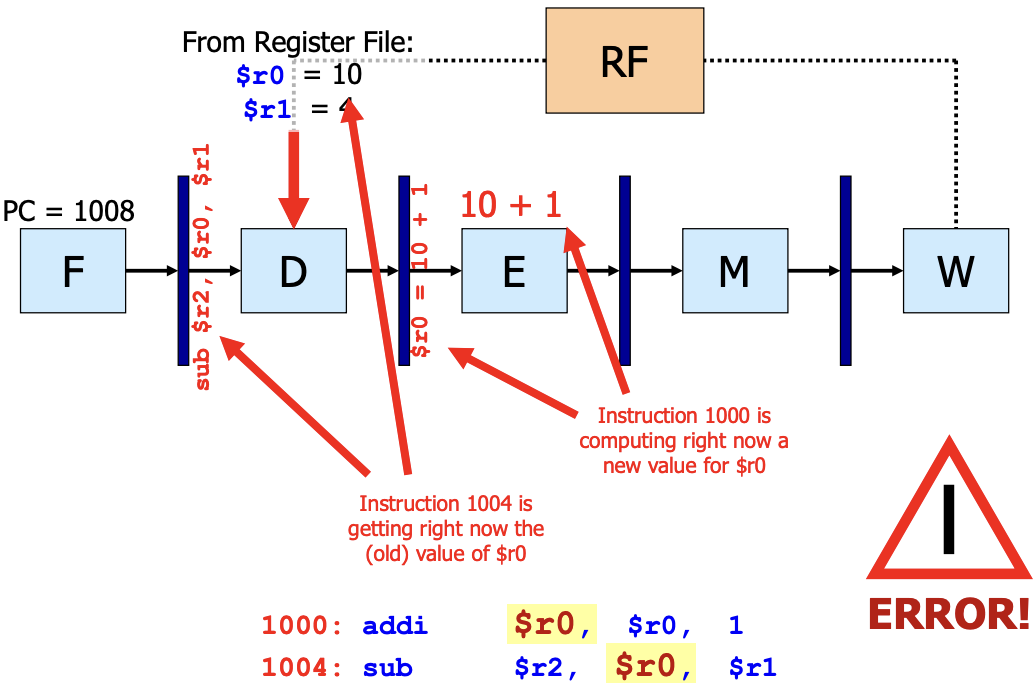
\includegraphics[width=0.55\textwidth]{chapters/chapter4c/images/problem.png}
\end{center}
Consider the following sequence of instructions executed in the previous example:
\begin{verbatim}
1000: addi $r0, $r0, 1
1004: sub $r2, $r0, $r1
\end{verbatim}

\begin{itemize}
    \item[-] At program counter (PC) 1000, the \texttt{addi} instruction modifies the value of register \texttt{\$r0} by incrementing it by 1.
    \item[-] At PC 1004, the \texttt{sub} instruction attempts to compute \texttt{\$r2} using the value of \texttt{\$r0}. However, it fetches the old value of \texttt{\$r0} from the register file because the result of the \texttt{addi} instruction is not yet available.
\end{itemize}

In this scenario, the \texttt{addi} instruction at PC 1000 is still in the \texttt{E} stage when the \texttt{sub} instruction at PC 1004 enters the \texttt{D} stage. Consequently, the \texttt{sub} instruction reads an outdated value of \texttt{\$r0}, leading to an incorrect result.

\section{Data Hazard Detection in Pipelined Processors}
Data hazards occur when instructions in a pipelined processor depend on the results of previous instructions that have not yet completed execution. To address this, the pipeline employs a hazard detection unit. The figure below illustrates the hazard detection mechanism for a sequence of instructions in a pipelined processor.

\begin{center}
    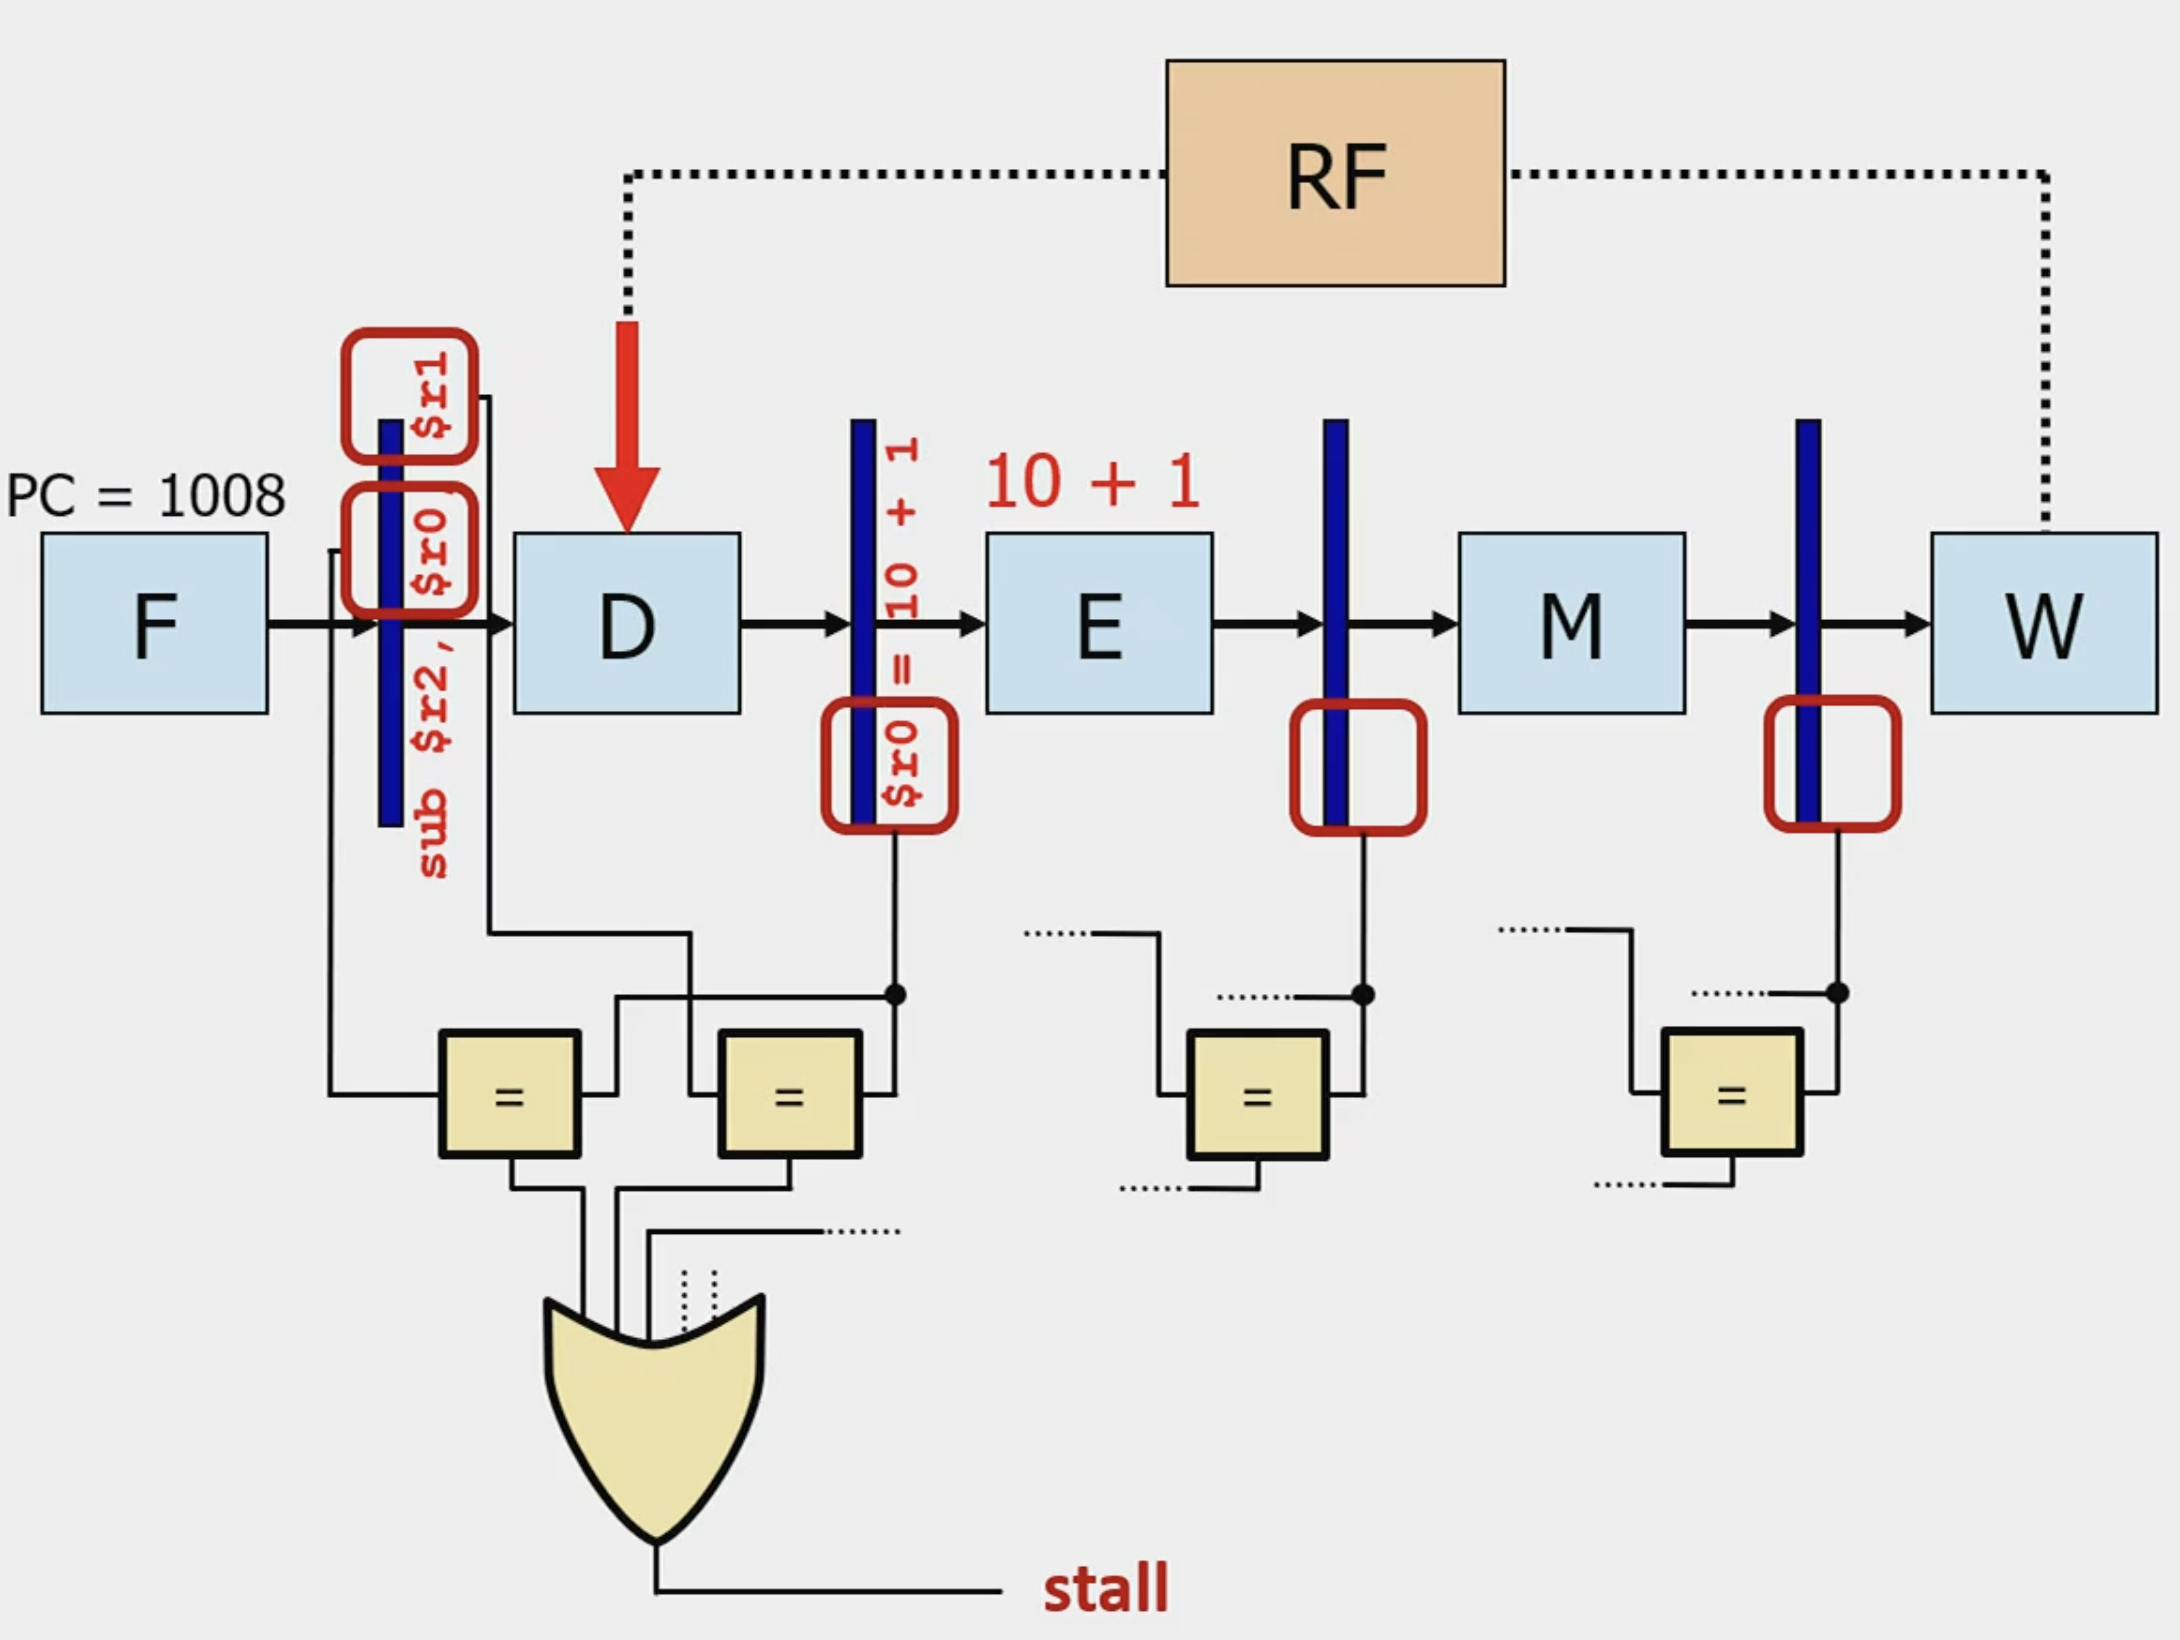
\includegraphics[width=0.45\textwidth]{chapters/chapter4c/images/detect.png}
\end{center}

In this example, a dependency exists between two instructions: the \texttt{sub} instruction in the Decode (D) stage requires the result of the \texttt{addi} instruction, which is still being processed in the Execute (E) stage. The hazard detection unit identifies this dependency and intervenes to maintain correct operation.

\subsection{Stalling in Instruction Execution}
Once a data hazard is detected, the pipeline resolves it using a stalling mechanism. This ensures that dependent instructions do not proceed until the required data becomes available. For the example discussed above, the stalling mechanism operates as follows:
\begin{center}
    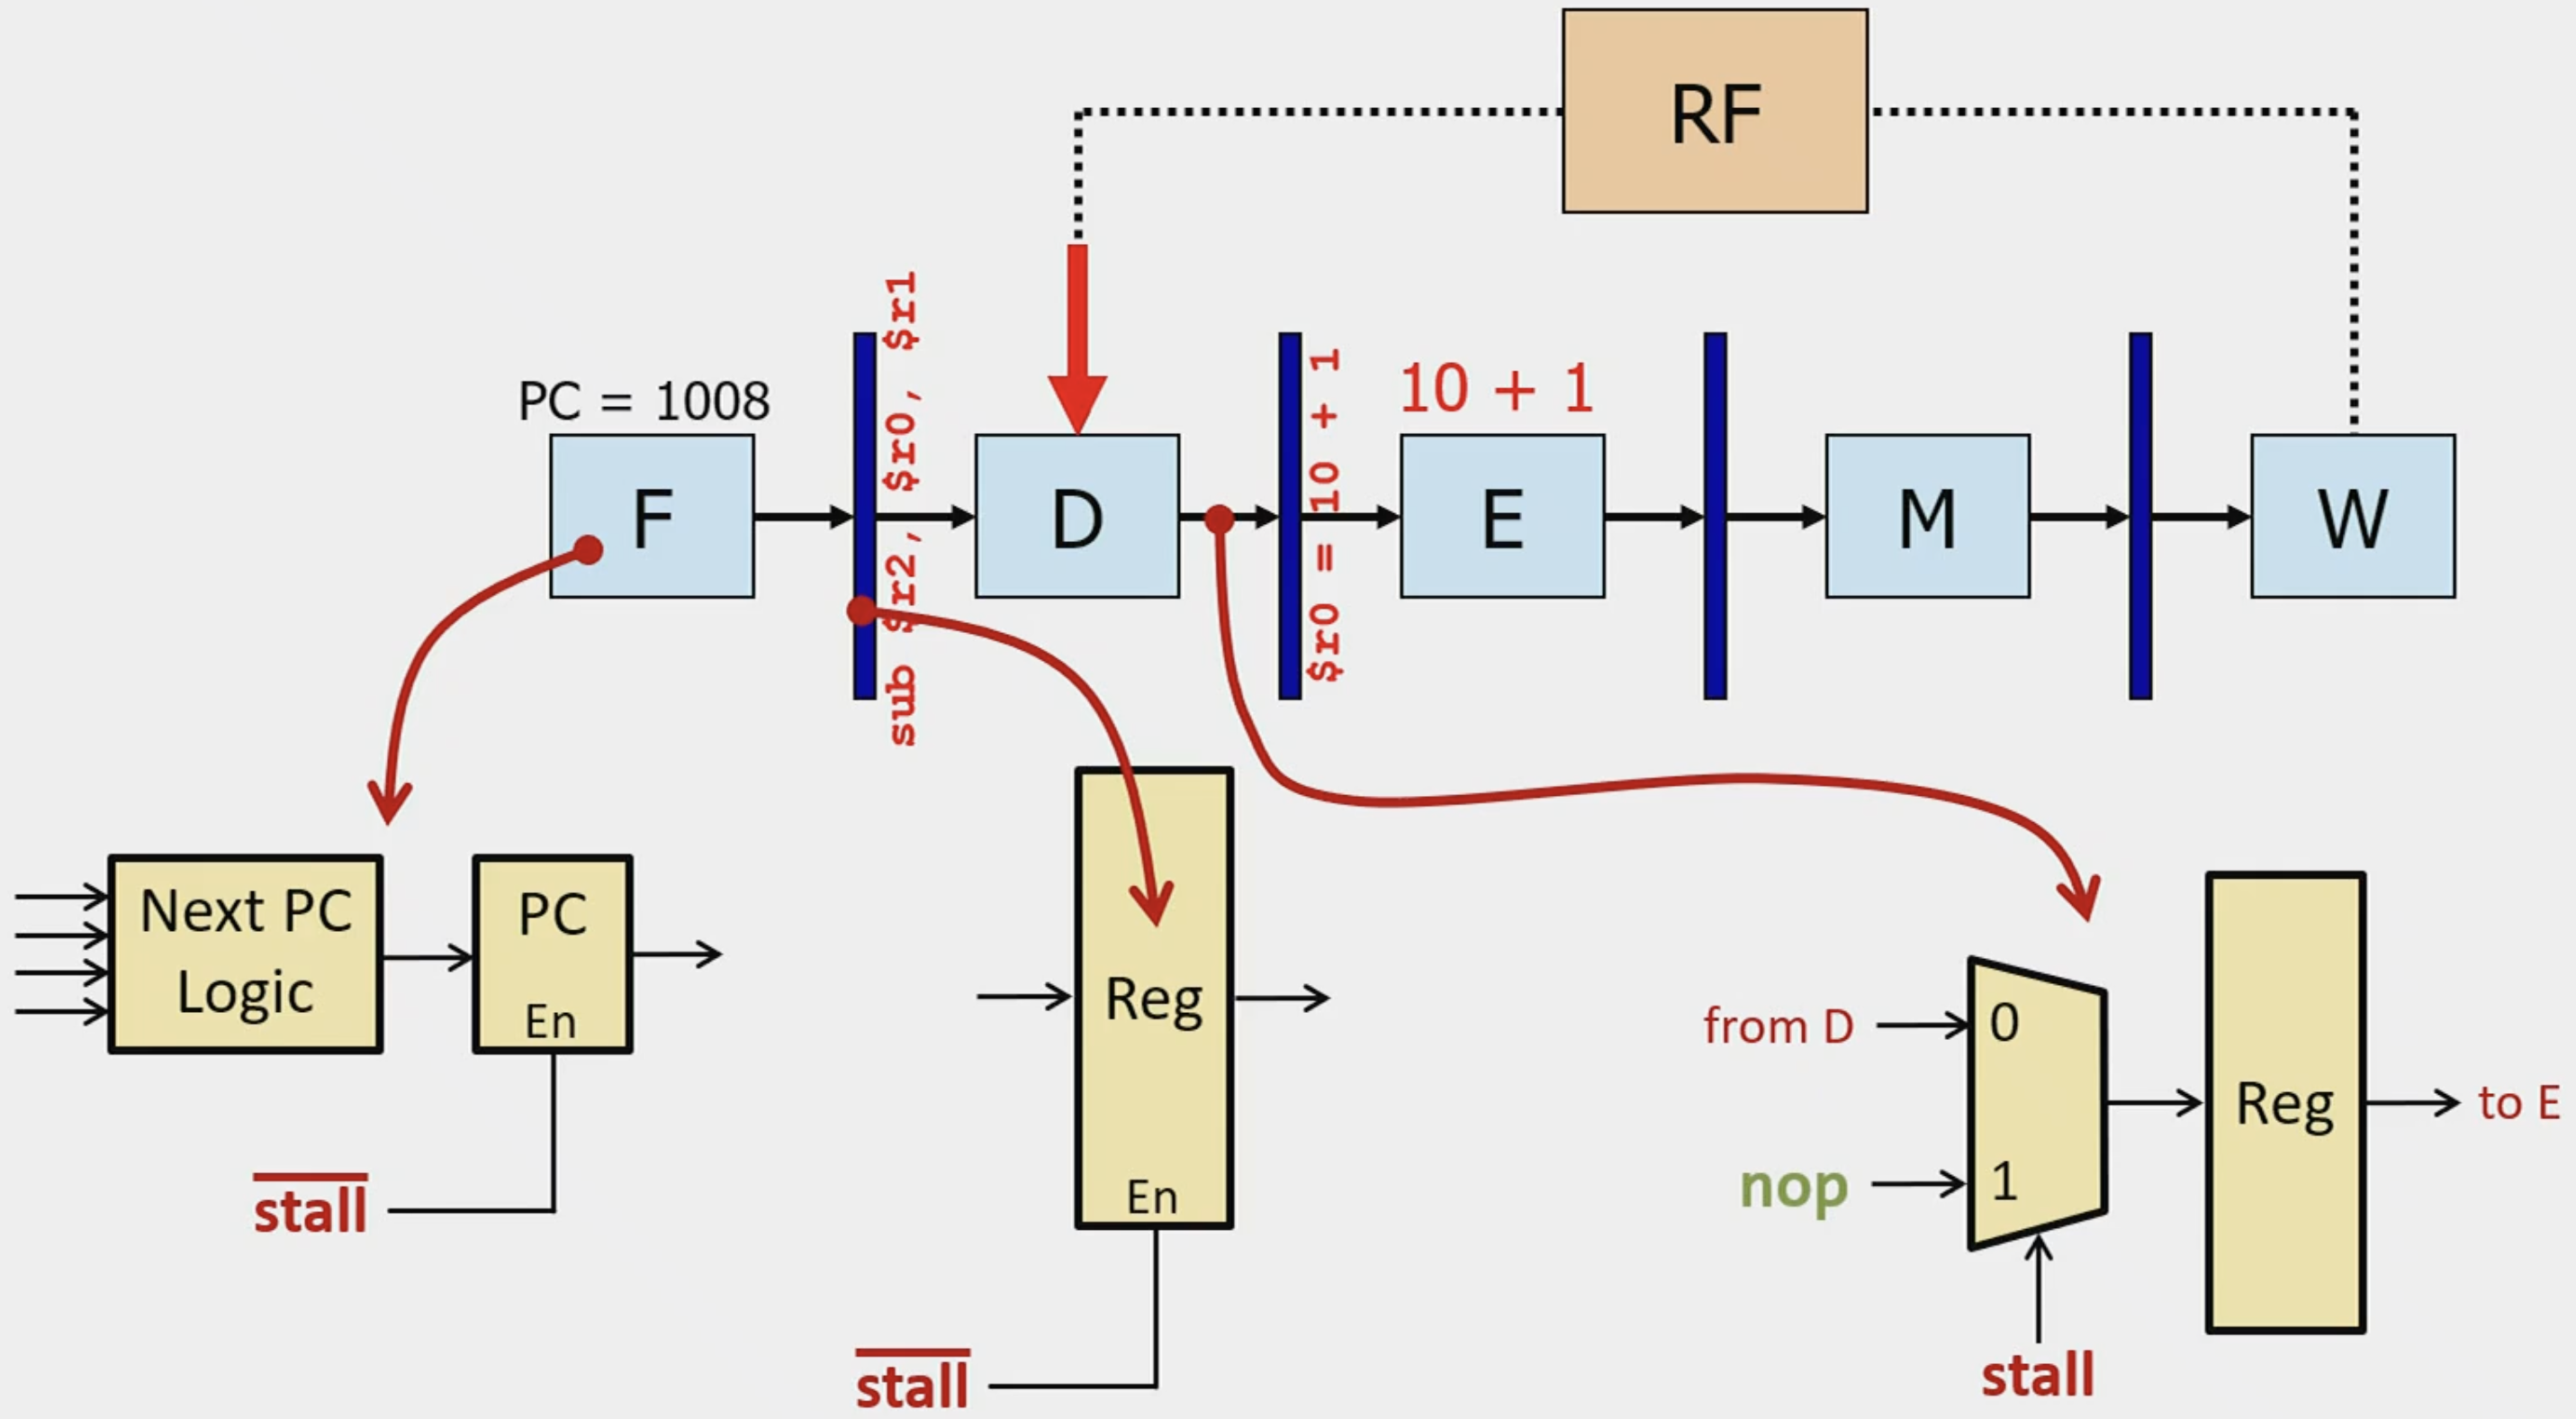
\includegraphics[width=0.65\textwidth]{chapters/chapter4c/images/stalling.png}
\end{center}
\subsubsection*{Stall Mechanism}
When the hazard detection unit identifies a data dependency, it triggers a stall in the pipeline to delay the dependent instruction until the required data becomes available. This is achieved as follows:
\begin{enumerate}
    \item The dependent instruction (e.g., \texttt{sub}) is held in the \textit{Decode (D)} stage until the instruction producing the required data (e.g., \texttt{addi}) computes its result in the \textit{Execute (E)} stage.
    \item A \texttt{nop} (no-operation) instruction is inserted into the pipeline to introduce a delay, allowing the producing instruction to complete its operation.
    \item The control logic halts the Program Counter (PC) and relevant pipeline registers temporarily to synchronize the execution flow.
\end{enumerate}

The flow of execution proceeds as follows:
\begin{itemize}
    \item The producing instruction progresses through the pipeline, computing its result in the \textit{E} stage.
    \item Simultaneously, the pipeline stalls the dependent instruction, holding it in the \textit{D} stage and inserting a \texttt{nop} in the \textit{Execute (E)} stage.
    \item Once the producing instruction writes its result to the register file, the dependent instruction resumes execution using the updated value.
\end{itemize}

While stalling reduces the overall throughput of the pipeline by introducing delays, it is essential for ensuring the correctness of computations. The hazard detection and stalling mechanism together provide a robust solution for managing data dependencies in pipelined processors.

\subsubsection{Conclusion}
By introducing stalling, the updated execution diagram is as follows:
\begin{center}
    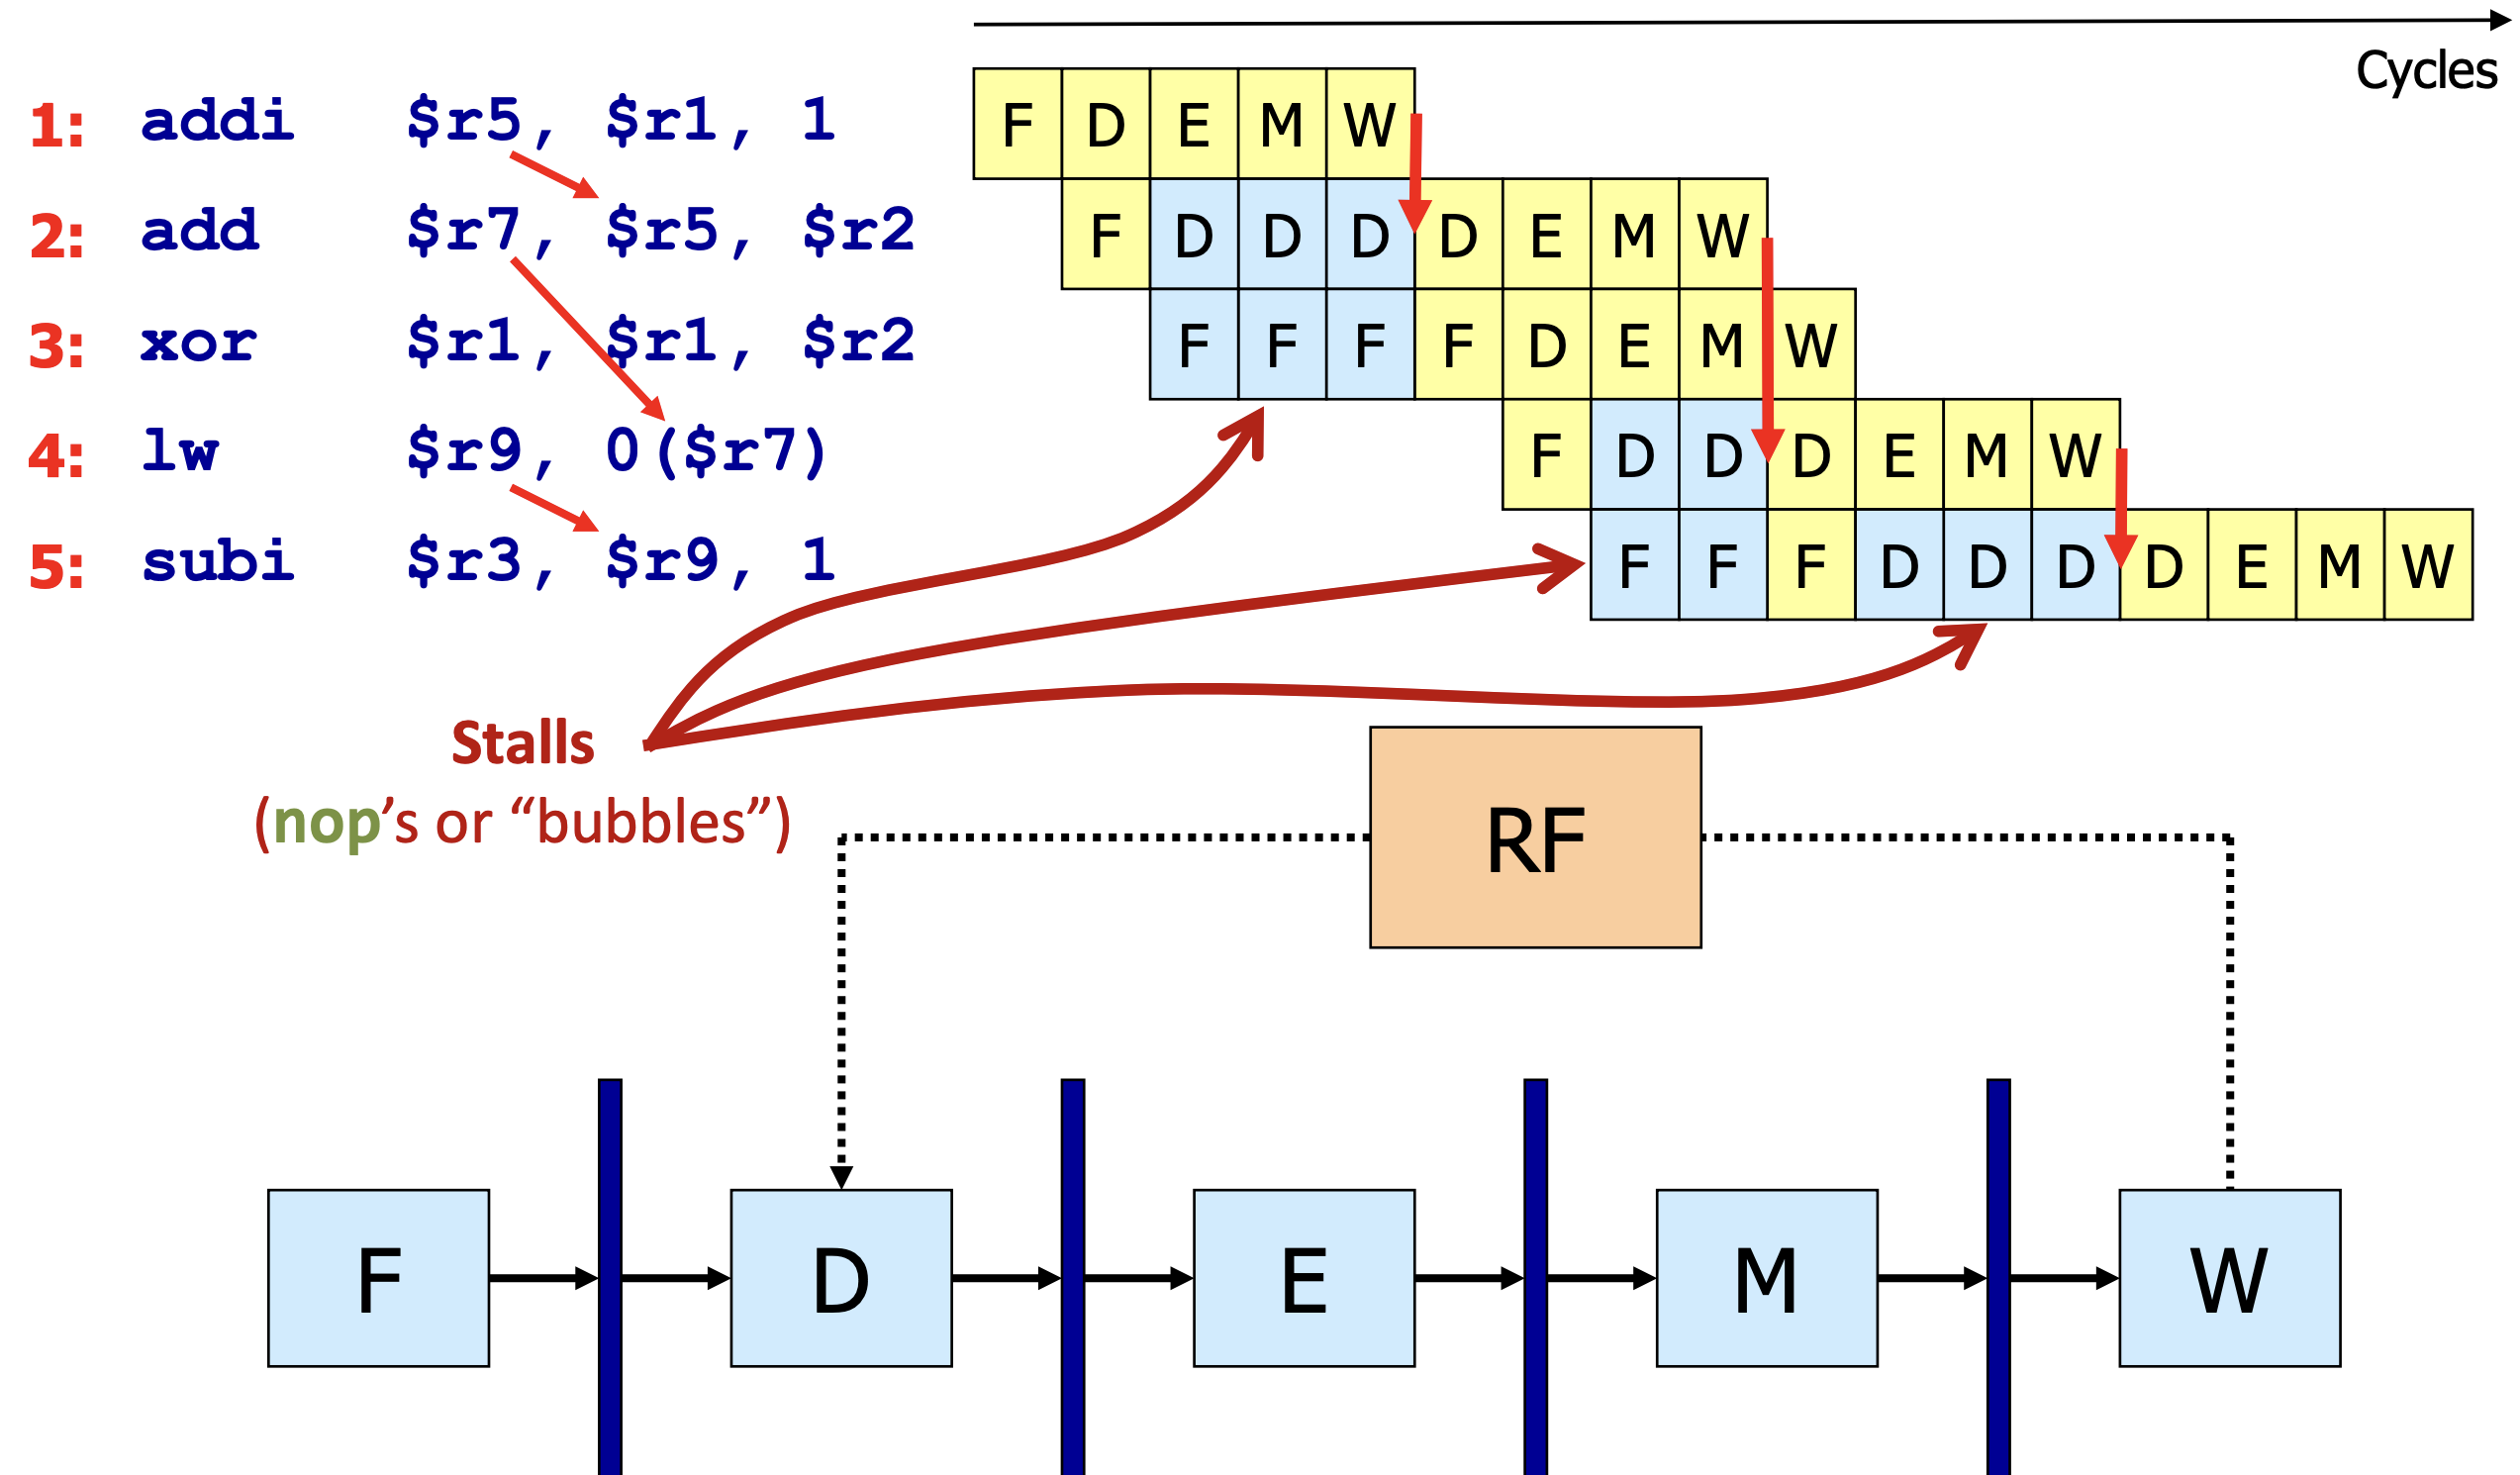
\includegraphics[width=0.65\textwidth]{chapters/chapter4c/images/diag.png}
\end{center}

\subsection{Alternative Solution}
An alternative approach to solving this problem could involve managing stalling in software. For instance, the compiler could statically insert the appropriate number of \texttt{nop} instructions before runtime to avoid any data hazards.
\begin{center}
    \includegraphics[width=0.65\textwidth]{chapters/chapter4c/images/solution2.png}
\end{center}
\newpage
\subsection{Data Hazards Resolved by Forwarding}
In pipelined processors, data hazards arise when an instruction depends on the result of a previous instruction that has not yet been written to the register file. Forwarding, also known as bypassing, is a hardware technique used to address this issue effectively.
\begin{center}
    \includegraphics[width=0.65\textwidth]{chapters/chapter4c/images/forwarding.png}
\end{center}
\begin{itemize}
    \item[-] \textbf{Timing vs. Location:} The required data becomes available at the correct time but is not in the necessary location for the dependent instruction.
    \item[-] \textbf{Direct Data Paths:} Forwarding paths are established to transfer data directly from one stage of the pipeline to another, eliminating unnecessary delays.
    \item[-] \textbf{Control Logic:} Additional circuitry, such as multiplexers, is employed to select the appropriate data input during the execute stage.
\end{itemize}

\noindent \textbf{Analogy:} \\
Imagine an assembly line in a factory where one worker produces a component needed by the next worker. Instead of waiting for the component to be placed in storage and then retrieved, the first worker directly hands it to the second worker. Similarly, forwarding allows data to be passed directly between pipeline stages without waiting for it to be written back to the register file.

\noindent \textbf{Example} \\
Consider the following two instructions:
\begin{verbatim}
    addi $r0, $r0, 1
    sub  $r2, $r0, $r1
\end{verbatim}
The result of the \texttt{addi} instruction must be used by the \texttt{sub} instruction. Without forwarding, the pipeline would have to wait until the \texttt{addi} result is written back to the register file before the \texttt{sub} instruction can proceed, causing a stall. With forwarding, the result from the \texttt{addi} instruction is directly sent to the execute stage of the \texttt{sub} instruction, allowing it to proceed without waiting.

\noindent \textbf{Implementation:} \\
The forwarding mechanism introduces hardware paths from:
\begin{itemize}
    \item The \textbf{Execute/Memory} pipeline register back to the Execute stage.
    \item The \textbf{Memory/Write-Back} pipeline register back to the Execute stage.
\end{itemize}
These paths are controlled to ensure that the correct data is provided to the execute stage when needed, bypassing the usual wait for the write-back phase and thereby maintaining the smooth flow of instructions through the pipeline.
\newpage
\subsection{Classic MIPS Pipeline with Forwarding}
\textit{Please take some time to understand this part, }
The classic MIPS pipeline consists of five stages:
\emph{Instruction Fetch}~(\textbf{F}),
\emph{Instruction Decode / Register Read}~(\textbf{D}),
\emph{Execute}~(\textbf{E}),
\emph{Memory Access}~(\textbf{M}),
and
\emph{Write Back}~(\textbf{W}). \\
Forwarding is a mechanism to resolve data hazards by enabling certain results to be directly passed between pipeline stages, bypassing the need for intermediate storage. When fully implemented, forwarding enables the following data paths:

\begin{center}
    \includegraphics[width=0.45\textwidth]{chapters/chapter4c/images/classic_mips.png}
\end{center}
\begin{itemize}
  \item \textbf{E $\rightarrow$ E:} The output from the Execute stage (\textbf{E}) of one instruction can be forwarded directly to the Execute stage of the next instruction, avoiding dependency-related stalls.
  \item \textbf{M $\rightarrow$ E:} The output from the Memory stage (\textbf{M}) can be forwarded to the Execute stage of the next instruction if required, bypassing the need to wait for the value to reach the Write Back stage.
  \item \textbf{W $\rightarrow$ D:} The output from the Write Back stage (\textbf{W}) can be supplied directly to the Decode stage (\textbf{D}) of a subsequent instruction during the same clock cycle.
\end{itemize}

\noindent
A notable special case is \emph{register-file forwarding} (\textbf{W $\rightarrow$ D}). In this scheme:
\begin{itemize}
  \item During the \textbf{W} stage, registers are written in the \textit{first half} of the clock cycle.
  \item During the \textbf{D} stage, registers are read in the \textit{second half} of the same cycle.
\end{itemize}
\noindent
This timing ensures that a register value written in \textbf{W} is immediately available for reading in \textbf{D}, avoiding a read-after-write hazard for consecutive instructions.

\noindent
In the classic MIPS pipeline, the forwarding paths described (\textbf{E $\rightarrow$ E}, \textbf{M $\rightarrow$ E}, \textbf{W $\rightarrow$ D}) are sufficient to resolve most data hazards. However, some instruction sequences may still require additional stall cycles if the needed forwarding path is unavailable.
\newpage
\section{Structural Hazards}

A \textbf{structural hazard} occurs when multiple instructions simultaneously require the same hardware resource (e.g., pipeline stage or memory port), potentially causing pipeline stalls or incorrect execution.

\begin{center}
\includegraphics[width=0.45\textwidth]{chapters/chapter4c/images/struct_hazard.png}
\end{center}

\subsubsection{Example}

Consider the following instruction sequence:

\begin{verbatim}
1. lw   $r0, 0($r1)      # Load word into $r0
2. lw   $r2, 4($r1)      # Load word into $r2
3. add  $r3, $r0, $r2    # Add $r0 and $r2, store in $r3
\end{verbatim}

In a pipelined processor with a single memory port, both \texttt{lw} instructions (1 and 2) attempt to access memory during the Memory (M) stage simultaneously. This conflict creates a structural hazard, forcing the processor to stall one instruction until the memory resource becomes available, thereby reducing throughput.

\subsubsection{Handling Cache Misses}

Cache misses can introduce structural hazards by stalling pipeline stages:

\begin{itemize}
    \item A miss in the Memory (M) stage can block access to memory or the bus, causing stalls in the Execute (E), Decode (D), and Fetch (F) stages.
\end{itemize}

\subsubsection{Stalling Strategies}

\begin{itemize}
    \item \textbf{Single Cache Miss}:
        \begin{itemize}
            \item Stall the Memory (M) stage and all preceding stages (E, D, F).
            \item Allow the Write-Back (W) stage to proceed to avoid blocking completed operations.
        \end{itemize}
    \item \textbf{Concurrent Misses}:
        \begin{itemize}
            \item Prioritize data cache misses over instruction cache misses to minimize overall stall time.
            \item This may temporarily cause resource contention on main memory.
        \end{itemize}
\end{itemize}

\subsubsection{Consequences of Unresolved Structural Hazards}

\begin{itemize}
    \item Instructions may execute out of order or prematurely, leading to resource conflicts.
    \item This can result in incorrect execution or pipeline corruption.
\end{itemize}

\subsubsection{Prevention in Our Pipeline}

\begin{itemize}
    \item Careful resource allocation ensures that structural hazards are \textbf{avoided}.
    \item Adequate provisioning of each pipeline stage and proper management of shared resources enable concurrent operation without contention.
\end{itemize}

\subsubsection{Dependency Example}

In the example above, the \texttt{sub} instruction depends on the result of the \texttt{lw} instruction (\$r0). If \$r0 is not ready when \texttt{sub} reaches the Execute stage, a structural hazard can occur unless stalls or forwarding mechanisms are implemented to handle the dependency.
\newpage
\section{Control Hazards in Pipelined Processors}

\subsection{The Problem}
A \emph{control hazard} (or \emph{branch hazard}) occurs in a pipelined CPU whenever the next instruction to fetch depends on the result of a branch. Since pipeline stages operate in parallel, the processor often fetches an instruction \emph{before} it knows whether the branch will be taken or not. If the branch is taken, the speculatively fetched instruction is wrong and must be \emph{flushed} (or invalidated); if the branch is not taken, execution continues normally.

\begin{center}
\textbf{Pipeline Stages:} F (Fetch), D (Decode), E (Execute), M (Memory), W (Write-back)
\end{center}

\subsubsection{Example}
\begin{verbatim}
Address   Instruction
----------------------------------
1000      beq   $r0, $r1, loop
1004      sub   $r2, $r0, $r1
1008      ...   (next instruction)
\end{verbatim}

When the CPU starts to fetch the instruction at \texttt{1004}, it may not yet know if the branch at \texttt{1000} is taken. If the branch is taken, the fetched instruction at \texttt{1004} is incorrect and must be discarded.

\subsection{Stalling (Flushing) the Pipeline}
One straightforward solution is to \emph{stall} the pipeline until it is known whether the branch will be taken. Conceptually:
\begin{enumerate}
  \item Fetch the branch instruction.
  \item Stall new instruction fetches until the branch outcome is computed (e.g., by the end of the E stage).
  \item If the branch is taken, jump to the correct target address; if not, continue with the sequential address.
\end{enumerate}
Stalling ensures correctness, but it \textbf{wastes several cycles} whenever a branch is encountered.

\begin{itemize}
  \item \textbf{Fetching \& Decoding a wrong instruction} is not harmful as long as it is not \emph{executed}.
  \item If the branch resolves in the E stage (cycle 3 for a 5-stage pipeline), two extra instructions may have been fetched speculatively. If the branch is taken, those two instructions are \emph{killed} (flushed); if not, they continue without delay.
\end{itemize}

\subsection{Delay Slots}
Another approach, historically used by MIPS and a few others, is to define \emph{delay slots} after a branch. In a 1-slot design:
\begin{enumerate}
  \item The instruction \emph{immediately} following the branch is always executed (the ``delay slot'').
  \item The branch effect (taken or not taken) occurs \emph{after} that delay slot instruction completes.
\end{enumerate}
Hence, the architecture enforces that instructions in the delay slot \emph{always} run, regardless of whether the branch is taken. In a 2-slot design, the next two instructions always execute, and so on.

\begin{center}
\textbf{Example of inserting NOPs (no-ops) in delay slots:}
\end{center}
\begin{verbatim}
1:   beq  $r0, $r1, loop  <-- branch
2:   nop                  <-- delay slot #1
3:   nop                  <-- delay slot #2
4:   sub $r2, $r0, $r1    <-- next real instruction
\end{verbatim}
While legal, using NOPs in delay slots merely shifts the stall problem into software. More sophisticated compilers attempt to move independent instructions into these slots so that the extra cycles are not wasted.


\section{Summary}

Pipelining in computer architecture can be hindered by three primary types of hazards:

\begin{itemize}
    \item \textbf{Data Hazards} (\textit{data dependences}): These occur when instructions depend on the results of previous instructions.
    \begin{itemize}
        \item \textit{Solutions:}
        \begin{itemize}
            \item Forwarding paths, wherever possible.
            \item Stalls, in all other cases.
        \end{itemize}
    \end{itemize}

    \item \textbf{Control Hazards} (\textit{jumps and branches}): These arise from the control flow of instructions, such as branches and jumps.
    \begin{itemize}
        \item \textit{Solutions:}
        \begin{itemize}
            \item Delay slots, if the architecture allows it.
            \item Branch prediction, to try to do the right thing.
            \item Stalls, if the above are not feasible.
        \end{itemize}
    \end{itemize}

    \item \textbf{Structural Hazards} (\textit{conflicting need for a resource}): These occur when multiple instructions require the same hardware resource simultaneously.
    \begin{itemize}
        \item \textit{Solutions:}
        \begin{itemize}
            \item Design rigid pipelines that avoid structural hazards by construction.
            \item Use stalls in cases where hazards cannot be avoided.
        \end{itemize}
    \end{itemize}
\end{itemize}
 
\chapter{Part IV(d) - Instruction Level Parallelism - Scheduling}
\section{Dynamic Scheduling and Out-of-Order Execution}
\label{sec:dynsched}

Modern processors often employ \textbf{dynamic scheduling} to exploit more instruction-level parallelism
(ILP). Instead of strictly following the program’s original instruction order
(\emph{in-order} execution), the processor can:

\begin{itemize}
  \item \textbf{Fetch and decode} instructions as early as possible, even if previous
        instructions have not completed.
  \item \textbf{Reorder} instruction execution to avoid idle functional units when
        long-latency instructions (e.g., divides) are in progress.
  \item \textbf{Ensure correctness} by respecting true data dependencies and properly
        writing results back in program order (via a \emph{Reorder Buffer (ROB)}).
\end{itemize}

\subsection{Motivating Example}
Consider the following sequence of floating-point operations:
\begin{verbatim}
  divd  $f0, $f2, $f4    # Long-latency division
  addd  $f10, $f0, $f8   # Depends on divd's result
  subd  $f12, $f8, $f14  # Independent of divd's result
\end{verbatim}

\begin{itemize}
  \item In a strict in-order pipeline, the \texttt{subd} could be stalled until
        \texttt{divd} completes its execution (because \texttt{addd} is waiting
        on \$f0).
  \item With dynamic scheduling, the processor can reorder
        \texttt{subd} before \texttt{addd} as soon as it identifies that
        \texttt{subd} does \emph{not} depend on \texttt{divd}.
  \item This reordering utilizes available resources without violating correctness.
\end{itemize}

\subsection{Breaking the Rigidity of Basic Pipelines}
In a standard five-stage pipeline (Fetch, Decode, Execute, Memory, Writeback),
stalls are common when earlier instructions hold resources or have unresolved
data dependencies. Dynamic scheduling mitigates these stalls by:
\begin{enumerate}
  \item \textbf{Continuing to fetch and decode} new instructions (even if some are
        stalled in execution).
  \item \textbf{Deferring writeback} until resources become available or dependencies
        are resolved, using dedicated hardware structures (e.g., reservation
        stations, reorder buffers).
  \item \textbf{Allowing out-of-order completion}: instructions finish as soon as they
        can, but their results are committed in-order to preserve program semantics.
\end{enumerate}

\subsection{Dynamically Scheduled Processor Overview}
A typical dynamically scheduled CPU integrates:
\begin{itemize}
  \item \textbf{Fetch/Decode} units that feed instruction information into
        \emph{reservation stations} (RS).
  \item Multiple functional units (ALU, FPU, Memory pipelines) operating in
        parallel.
  \item A \textbf{Reorder Buffer (ROB)} to track instruction completion and to
        ensure in-order retirement (commit) of results.
  \item \textbf{Forwarding paths} to provide operands directly to waiting instructions
        without requiring all results to be written back to the register file first.
\end{itemize}

By decoupling instruction fetch/decode from their actual execution, a
\textbf{dynamically scheduled processor} allows more effective use of hardware
resources and improves overall performance, particularly for workloads with
long-latency operations or frequent stalls in in-order pipelines.
\subsection{Reservation Stations}

Reservation stations are hardware queues that temporarily hold instructions before they are sent to an execution unit. They are a key component in enabling \textbf{out-of-order execution} within a processor. This mechanism allows the CPU to execute instructions as soon as their necessary resources are available, rather than strictly adhering to the program's original order.

\subsubsection{How Reservation Stations Work}

Reservation stations facilitate several critical functions in the CPU:

\begin{enumerate}
    \item \textbf{Check Operand Availability:}
    They verify that all input operands required by an instruction have been computed and are available, either in the register file or through bypassing from another execution unit.

    \item \textbf{Prevent Structural Hazards:}
    They ensure that the targeted execution unit is free and ready to accept a new operation, thereby avoiding conflicts over shared functional units.

    \item \textbf{Enable Dynamic Scheduling:}
    They allow instructions to be dispatched to available execution units as soon as both their operands and the necessary functional resources are ready, rather than waiting for earlier instructions to complete.
\end{enumerate}

\subsubsection{Components of a Reservation Station}

Each entry within a reservation station typically contains the following elements:

\begin{itemize}
    \item \textit{Operation Code} (e.g., \texttt{add}, \texttt{sub}, \texttt{mul}): Specifies the operation to be performed.
    \item \textit{Operands or Tags}: Contains the actual operands needed for the operation or tags that reference future instructions responsible for producing those operands.
    \item \textit{Status Bits}: Indicate whether the operands are ready and whether an appropriate execution unit has been reserved.
\end{itemize}

\subsubsection{Execution Process}

\begin{enumerate}
    \item \textbf{Issuing Instructions:} When an instruction enters a reservation station, it waits until both its operands are available and the required execution unit is free.
    \item \textbf{Executing Instructions:} Once these conditions are met, the reservation station issues the instruction to the execution unit.
    \item \textbf{Broadcasting Results:} After execution, the result is forwarded to all reservation stations that are waiting for that particular value, updating their entries to reflect that the operand is now valid.
\end{enumerate}

\begin{center}
    \includegraphics[width=0.65\textwidth]{chapters/chapter4d/images/reservation_table.png}
\end{center}

\subsubsection{Analogy: Kitchen Order Management}

Think of reservation stations as a \textbf{kitchen's order management system} in a restaurant:

\begin{itemize}
    \item \textbf{Orders as Instructions:} Each customer's order is an instruction that needs to be prepared.
    \item \textbf{Ingredients as Operands:} The ingredients required for each dish represent the operands. An order can only be prepared if all necessary ingredients are available.
    \item \textbf{Chefs as Execution Units:} The chefs are the execution units that prepare the dishes.
\end{itemize}

\textbf{Process Flow:}
\begin{enumerate}
    \item \textbf{Taking Orders:} Orders are placed in the reservation station (waiting area) as they come in.
    \item \textbf{Checking Ingredients:} The system verifies that all ingredients for an order are available.
    \item \textbf{Assigning to Chefs:} If ingredients are ready and a chef is available, the order is handed off to the chef for preparation.
    \item \textbf{Updating Availability:} Once a dish is prepared, the result is available to fulfill other orders that might depend on it.
\end{enumerate}

\subsubsection{Summary}
Reservation stations decouple the dispatching of instructions from the availability of their operands and the execution units. By doing so, they enhance the processor's ability to execute instructions out of order, thereby improving overall performance and efficiency.

\subsection{Register Renaming and Data Dependencies}
Register renaming is a technique used to eliminate \textbf{Write-After-Write (WAW)} and \textbf{Write-After-Read (WAR)} dependencies, collectively referred to as \textit{name dependencies}. These dependencies occur because registers are reused across multiple instructions, despite the absence of actual data flow between them.

\subsubsection{Pipeline Hazards and Dependency Types}

Pipeline execution is prone to the following dependencies:
\begin{itemize}
    \item \textbf{Read-After-Write (RAW):} True data dependence, where an instruction requires the output of a previous one.
    \item \textbf{Write-After-Write (WAW):} Name dependence, resolved by renaming.
    \item \textbf{Write-After-Read (WAR):} Name dependence, resolved by renaming.
\end{itemize}

In dynamic pipelines, out-of-order execution can introduce hazards like WAW and WAR. Renaming ensures correctness by maintaining unique register identifiers, enabling both in-order and out-of-order pipelines to avoid conflicts.

\subsubsection{Example}

Consider the following instructions:\\
\begin{minipage}[t]{0.45\textwidth}
    \begin{verbatim}
        divd  $f0, $f1, $f2
        addd  $f3, $f0, $f4
        subd  $f4, $f5, $f6
        adddi $f0, $f5, 10
    \end{verbatim}
    - \texttt{addd} has a \textbf{RAW} dependence on \texttt{divd}. \\
    - \texttt{subd} has a \textbf{WAR} dependence on \texttt{addd}. \\
    - \texttt{adddi} has a \textbf{WAW} dependence on \texttt{divd}. \\
\end{minipage}
\hfill
\vline
\hfill
\begin{minipage}[t]{0.45\textwidth}
    By renaming, these dependencies are resolved:
    \begin{verbatim}
        divd  $f0, $f1, $f2
        addd  $f3, $f0, $f4
        subd  $f30, $f5, $f6
        adddi $f29, $f30, 10
    \end{verbatim}
\end{minipage} \\ \vspace{10px}
\textbf{This ensures the pipeline executes efficiently without conflicts, improving instruction throughput.}

\newpage
\section{Dynamically Scheduled Processor}
A \emph{dynamically scheduled processor} uses hardware mechanisms to exploit
\emph{out-of-order} execution, allowing instructions to proceed as soon as
their operands become available. This contrasts with a strictly pipelined MIPS
design, where all instructions flow in \emph{order} through the five pipeline
stages (F, D, E, M, W). By dynamically scheduling instructions, the
processor can reduce stalls and more effectively utilize hardware resources.

\begin{center}
    \includegraphics[width=0.65\textwidth]{chapters/chapter4d/images/complete.png}
\end{center}
\begin{itemize}
  \item[-] \textbf{Instruction Fetch \& Decode Unit:}
    Fetches and decodes instructions, dispatching them to the appropriate
    \emph{reservation stations} once the instruction type is identified.

  \item[-] \textbf{Reservation Stations:}
    Buffers that hold instructions waiting for the required operands or
    execution unit to become available. Each functional unit (e.g., ALU,
    floating-point, branch, or load/store) typically has its own set of
    reservation stations.

  \item[-] \textbf{ALU, FP Unit, Branch Unit, Load/Store Unit:}
    Execution units where instructions are actually carried out. The Load/Store
    Unit also manages memory operations. Because these units operate in parallel,
    multiple independent instructions can be serviced simultaneously.

  \item[-] \textbf{Register File:}
    Stores the architectural registers. Instructions read from and write to
    this file (potentially out of program order), but the final states are
    committed in order, preserving correct program semantics.

  \item[-] \textbf{Commit Unit:}
    Also referred to as the \emph{retirement} or \emph{write-back stage}. It
    ensures that the processor's \emph{architectural state} is updated in the
    correct program order, even though internal execution may be out of order.
\end{itemize}

\subsubsection*{Example Execution}
Suppose we have the following sequence of instructions:
\[
\begin{aligned}
&I1: \text{R1} \leftarrow \text{R2} + \text{R3}\\
&I2: \text{R4} \leftarrow \text{R1} \times \text{R5}\\
&I3: \text{R6} \leftarrow \text{R7} + \text{R8}
\end{aligned}
\]
In a strictly pipelined MIPS processor, \(\text{I2}\) would have to stall
while waiting for \(\text{R1}\) (produced by \(\text{I1}\)) to be written back.
However, a dynamically scheduled processor can place \(\text{I2}\) into a
reservation station, and simultaneously issue \(\text{I3}\) to the ALU,
because \(\text{I3}\) does not depend on \(\text{I1}\) or \(\text{I2}\).
This allows overlapping execution and reduced idle cycles.
\newpage
\subsection{Precise vs.\ Imprecise Exceptions}
Exceptions occur when the processor encounters an event requiring special handling (e.g., page fault, unsupported instruction).
They can be categorized as \emph{precise} or \emph{imprecise} based on whether the exact instruction that caused the exception---and the architectural state associated with that point in the instruction stream---can be precisely identified.

\begin{itemize}
  \item \textbf{Precise Exceptions}
  \begin{itemize}
    \item The processor enforces an in-order view of instruction completion at the point of the exception.
    \item This implies that all instructions before the faulting instruction have completed, and none of the subsequent instructions have begun or altered the architectural state.
    \item Reordering or out-of-order execution may still happen internally, but when an exception occurs, the processor ``commits'' instructions in a way that appears strictly in-order.
    \item This behavior simplifies error handling, as the operating system (OS) or exception handler knows exactly where the problem occurred and which instructions completed.
  \end{itemize}
  \item \textbf{Imprecise Exceptions}
  \begin{itemize}
    \item Out-of-order execution becomes visible to the user (or OS), meaning the faulting instruction might not be clearly identified at the time of the exception.
    \item The OS or programmer must assume that instructions have partially or fully executed in a different order than expected.
    \item Correcting the architectural state becomes more complex; the system may need to re-execute an entire subroutine to ensure correctness.
    \item Modern architectures generally avoid imprecise exceptions because of these complexities (especially for critical features such as virtual memory or I/O).
  \end{itemize}
\end{itemize}

\subsubsection{Out-of-Order Commitment and Exceptions}
Dynamic (out-of-order) execution complicates exception handling because the processor may complete some instructions after the faulting instruction if it issued them early. In a precise exception model, the hardware automatically rolls back or defers the effects of later instructions so that:
%
\begin{enumerate}
  \item Everything before the faulting instruction is guaranteed to have completed.
  \item No instructions after the faulting instruction have committed any state.
\end{enumerate}

This exact commitment model allows the exception handler to identify the precise location of the fault. When exceptions are imprecise, the program may need to be restarted from an earlier point to restore correct state, making it challenging for both the hardware and software to manage.

\newpage
\subsection{Reordering Instructions at Writeback}
A \emph{reorder buffer} (ROB) is used in out-of-order processors to maintain correct program order when writing back results to the architectural register file and memory. While instructions may execute in parallel or out of order, the ROB ensures that their visible effects (writes to registers/memory) occur in the original program order. This mechanism preserves the logical behavior of the program while also taking advantage of pipeline parallelism.
\begin{center}
    \includegraphics[width=0.65\textwidth]{chapters/chapter4d/images/rob.png}
\end{center}
\subsubsection{High-Level Overview.}
\begin{itemize}
  \item \textbf{Out-of-Order Execution:} After fetching and decoding, instructions are dispatched to execution units as soon as their operands become available. This enables the processor to exploit instruction-level parallelism.
  \item \textbf{Reorder Buffer (ROB):} Each fetched instruction is allocated an entry in the ROB. The entry holds:
    \begin{enumerate}
      \item The instruction’s \emph{program counter} (PC) and a unique \emph{tag}.
      \item The \emph{destination} (register or memory address).
      \item The \emph{result} value (once the execution unit produces it).
      \item An \emph{exception status} field to indicate whether an exception occurred.
    \end{enumerate}
  \item \textbf{Writeback \& Commit:} Although execution finishes out of order, the ROB enforces an \emph{in-order} commit. The oldest (head) entry in the ROB is checked first:
    \begin{enumerate}
      \item If its result is ready and no exception has occurred, the commit unit writes the result to the destination register or memory location.
      \item The ROB entry is then freed, and the \emph{head} pointer moves to the next instruction.
    \end{enumerate}
  \item \textbf{Preserving Program Correctness:} If an exception flag is set for the head entry, the pipeline can be flushed and the exception handled in program order, ensuring correct state recovery.
\end{itemize}

\subsubsection{Execution Steps.}
\begin{enumerate}
  \item \emph{Fetch \& Decode:} Instructions are fetched in program order and assigned entries in the ROB. Each ROB entry records necessary metadata (PC, destination, etc.).
  \item \emph{Dispatch to Execution Units:} As soon as sources for an instruction are ready, it can be sent to an available execution unit. Meanwhile, the ROB entry remains allocated to that instruction.
  \item \emph{Receive Results in ROB:} Once an execution unit finishes, it writes the result (along with the instruction’s tag) back to the ROB. The destination register or memory is \emph{not} updated yet.
  \item \emph{Commit in Program Order:} The reorder buffer’s head entry is checked:
    \begin{itemize}
      \item If the head instruction’s result is available and no exception is flagged, that value is \emph{committed} to the architectural register file or memory in correct program order.
      \item The head pointer is advanced, retiring the entry from the ROB.
      \item This process repeats as subsequent instructions at the head become ready and valid.
    \end{itemize}
\end{enumerate}

\subsubsection{Why It Improves Performance.}
Even though instructions are effectively \emph{reordered} before the final writeback, the pipeline overlaps multiple steps of different instructions. The reorder buffer allows:
\begin{itemize}
  \item[-] \textbf{Parallel Execution:} Independent instructions execute simultaneously in different pipeline stages, reducing overall latency.
  \item[-] \textbf{Hazard Resolution:} The ROB tracks which instructions have completed and can manage data hazards by forwarding results as soon as they are produced.
  \item[-] \textbf{In-Order Commit Guarantee:} The programmer-visible state updates in strict order (the ROB’s head-to-tail sequence), preserving correct semantics without stalling earlier instructions for later ones.
\end{itemize}

Thus, the reorder buffer provides the illusion of in-order execution while allowing out-of-order performance gains. As soon as an instruction completes, its result is available for subsequent instructions; however, to ensure correctness, final commitment of these results to the architectural state occurs strictly in the order of the original program.
\newpage
\section*{Dynamically Scheduled Processor: Step-by-Step Execution}
\vspace{-5px}
This outlines the operation of a dynamically scheduled processor, broken down into modular stages that can be adapted for various design choices (e.g., with or without forwarding paths, reservation stations, etc.). Each step is presented using a structured \textbf{if-then-else} format and emphasizes how instructions flow through the pipeline under different conditions. \\
\textit{Basically an algorithm to answer this chapter's exercises.}
\vspace{-15px}
{
  % Set spacing adjustments for lists
  \setlist{noitemsep, topsep=1pt}
  % Reduce font size locally
  \small
  \subsubsection*{1. Instruction Fetching}
  \vspace{-5px}
  \begin{enumerate}
      \item \textbf{Fetch Attempt}
      \begin{itemize}
          \item \textbf{IF} the instruction cache (I-cache) is ready to serve a new instruction \textbf{THEN}
          \begin{itemize}
              \item Fetch the next instruction address from the Program Counter (PC).
              \item Send the address request to the I-cache.
              \item Increment or update PC for the next instruction (or branch target if known).
          \end{itemize}
          \item \textbf{ELSE} (\emph{I-cache miss} or \emph{pipeline stall condition})
          \begin{itemize}
              \item Stall the fetch stage until the I-cache responds, or the pipeline is cleared.
          \end{itemize}
      \end{itemize}
      \item \textbf{Branch Misprediction Handling}
      \begin{itemize}
          \item \textbf{IF} a branch misprediction is detected \textbf{THEN}
          \begin{itemize}
              \item Flush the fetched instructions after the mispredicted branch.
              \item Update PC with the correct branch target.
              \item Re-fetch instructions from the correct location.
          \end{itemize}
          \item \textbf{ELSE}
          \begin{itemize}
              \item Continue normal fetching.
          \end{itemize}
      \end{itemize}
  \end{enumerate}
  \vspace{-15px}
  \subsubsection*{2. Instruction Decoding}
  \vspace{-5px}
  \begin{enumerate}
      \item \textbf{Decode Phase}
      \begin{itemize}
          \item \textbf{IF} the decode (or dispatch) hardware and any necessary pipeline registers are available \textbf{THEN}
          \begin{itemize}
              \item Read the fetched instruction.
              \item Decode the opcode and identify operands and destination register(s).
          \end{itemize}
          \item \textbf{ELSE}
          \begin{itemize}
              \item Stall decode until resources become free.
          \end{itemize}
      \end{itemize}
      \item \textbf{Hazard Checks}
      \begin{itemize}
          \item \textbf{IF} there is a structural hazard (e.g., decode hardware busy) \textbf{THEN}
          \begin{itemize}
              \item Stall the decode stage until the hazard is cleared.
          \end{itemize}
          \item \textbf{IF} there is a data hazard (register not yet available or pending in the Reorder Buffer) \textbf{THEN}
          \begin{itemize}
              \item Mark the instruction as needing operands from future writes or forwarding paths.
          \end{itemize}
          \item \textbf{ELSE}
          \begin{itemize}
              \item Proceed to place the instruction into an appropriate reservation station.
          \end{itemize}
      \end{itemize}
  \end{enumerate}
  \vspace{-15px}
  \subsubsection*{3. Reservation Stations}
  \vspace{-5px}
  \begin{enumerate}
      \item \textbf{Instruction Buffering and Dependency Resolution}
      \begin{itemize}
          \item \textbf{IF} a reservation station matching the instruction type (ALU, FP, Branch, or Load/Store) is free \textbf{THEN}
          \begin{itemize}
              \item Place the instruction in the station, along with operand tags or values.
              \item Check which operands are currently valid (available in the register file, or forwarded) and which are pending.
          \end{itemize}
          \item \textbf{ELSE}
          \begin{itemize}
              \item Stall the instruction until a reservation station becomes available.
          \end{itemize}
      \end{itemize}
      \item \textbf{Operand Availability}
      \begin{itemize}
          \item \textbf{IF} all input operands are ready \textbf{THEN}
          \begin{itemize}
              \item Dispatch the instruction to the appropriate execution unit immediately.
          \end{itemize}
          \item \textbf{ELSE}
          \begin{itemize}
              \item Wait for forwarding signals or for the Reorder Buffer (ROB) to broadcast the result.
          \end{itemize}
      \end{itemize}
  \end{enumerate}
  \newpage
  \subsubsection*{4. Execution Units}
  \vspace{-5px}
  \begin{enumerate}
      \item \textbf{Instruction Execution}
      \begin{itemize}
          \item \textbf{IF} the execution unit is free and all operands are valid \textbf{THEN}
          \begin{itemize}
              \item Execute the instruction (e.g., perform ALU operation, load/store, floating-point operation, or branch evaluation).
          \end{itemize}
          \item \textbf{ELSE}
          \begin{itemize}
              \item Stall in the reservation station until the execution unit is available and any missing operands are forwarded.
          \end{itemize}
      \end{itemize}
      \item \textbf{Forwarding and ROB Updates}
      \begin{itemize}
          \item \textbf{IF} the processor supports forwarding \textbf{THEN}
          \begin{itemize}
              \item Immediately broadcast the result on the Common Data Bus (CDB) so dependent instructions can receive the value without waiting for it to be written to the register file.
          \end{itemize}
          \item \textbf{ELSE}
          \begin{itemize}
              \item Write the result into the reorder buffer and/or register file.
              \item Dependent instructions must wait until the write is complete to read the result.
          \end{itemize}
      \end{itemize}
  \end{enumerate}
  \vspace{-15px}
  \subsubsection*{5. Commit Unit}
  \vspace{-5px}
  \begin{enumerate}
      \item \textbf{Reorder Buffer (ROB) and In-Order Commit}
      \begin{itemize}
          \item \textbf{IF} the instruction is at the head of the ROB and has completed execution with no exceptions \textbf{THEN}
          \begin{itemize}
              \item Commit the result to the architectural register file or memory (for store operations).
              \item Remove the instruction entry from the ROB.
          \end{itemize}
          \item \textbf{ELSE} (\emph{instruction not yet at head of ROB} or \emph{exception detected})
          \begin{itemize}
              \item Stall the commit stage until the head instruction is fully ready.
              \item \textbf{IF} an exception or misprediction is detected \textbf{THEN}
              \begin{itemize}
                  \item Flush instructions in the ROB after the faulting or mispredicted instruction.
                  \item Recover architectural state from the last known good state or from checkpoints.
              \end{itemize}
          \end{itemize}
      \end{itemize}
  \end{enumerate}
  \vspace{-15px}
  \subsubsection*{6. Register File}
  \vspace{-5px}
  \begin{enumerate}
      \item \textbf{Register Access and Dynamic Scheduling Support}
      \begin{itemize}
          \item \textbf{IF} the result is not yet committed (i.e., it resides in the ROB) \textbf{THEN}
          \begin{itemize}
              \item Dependent instructions obtain the result from forwarding paths or by listening to the ROB broadcast.
          \end{itemize}
          \item \textbf{ELSE}
          \begin{itemize}
              \item Read the committed value from the register file in the usual manner.
          \end{itemize}
      \end{itemize}
  \end{enumerate}
  \vspace{-15px}
  \subsubsection*{7. Execution Scenarios (Decision Tree)}
  \vspace{-5px}
  \noindent
  \textbf{Scenario 1: With Forwarding Paths}
  \begin{enumerate}
      \item \textbf{IF} an instruction completes in the execution unit
      \begin{itemize}
          \item \textbf{THEN} broadcast the result immediately to all reservation stations listening for that tag.
          \item Dependent instructions that had this operand pending can now proceed to execution in the next cycle (if their other operands are also ready and an execution unit is free).
      \end{itemize}
  \end{enumerate}
  \noindent
  \textbf{Scenario 2: Without Forwarding Paths}
  \begin{enumerate}
      \item \textbf{IF} an instruction completes in the execution unit
      \begin{itemize}
          \item \textbf{THEN} the result is first written to the reorder buffer (and eventually to the register file).
          \item Dependent instructions wait until the value is visible in the register file or the ROB can broadcast the commitment.
      \end{itemize}
  \end{enumerate}

  \textit{Lastly, general rule, if something is busy, or if it doesn't have enough space to add an instruction/operation etc\dots, Stall.}\vspace*{-10px}
  \subsubsection*{8. Performance Comparison}
  \vspace{-5px}
  \begin{itemize}
      \item Dynamic scheduling allows multiple instructions to be \textit{in-flight}, decoding and executing out of order as their operands become available.
      \item \textbf{Compared to a simple in-order pipeline}:
      \begin{itemize}
          \item More instructions can execute in parallel if they do not depend on each other.
          \item Hazards are resolved dynamically, leading to fewer pipeline stalls.
          \item Forwarding paths further reduce stalls by providing immediate data to dependent instructions.
      \end{itemize}
      \item Overall, the utilization of hardware resources is improved and throughput (instructions per cycle) is increased.
  \end{itemize}
} 
\chapter{Part 4f: Instruction Level Parallelism (ILP) Besides and Beyond Superscalars}

Instruction-Level Parallelism (ILP) is the measure of how many operations in a computer program can be performed simultaneously. The goal of ILP is to exploit parallel execution within a single thread to improve performance. Traditional \emph{superscalar} architectures achieve ILP by issuing multiple instructions in one clock cycle, but new challenges arise when hardware and program behavior limit the amount of parallelism that can be extracted.

\section{Superscalar Execution}
Modern high-performance processors often implement \emph{superscalar} execution, where multiple instructions are issued (i.e., started) in the same clock cycle to increase throughput. However, to realize sustained parallelism, several requirements must be met:

\begin{center}
    \includegraphics[width=0.45\textwidth]{chapters/chapter4f/images/superscalar.png}
\end{center}

\begin{itemize}
  \item \textbf{Fetch more instructions per cycle.}\\
  An instruction cache with sufficient bandwidth is needed to supply multiple instructions each cycle. Without adequate fetch capacity, the pipeline stalls and cannot exploit superscalar capabilities.

  \item \textbf{Commit more instructions per cycle.}\\
  To retire (commit) multiple instructions per cycle, the \emph{reorder buffer} (ROB) and the \emph{register file} must have enough ports and resources. A lack of commit bandwidth creates a bottleneck, undoing the benefits of parallel execution in earlier stages.

  \item \textbf{Obey data and control dependencies.}\\
  Even if hardware can fetch and commit multiple instructions per cycle, \emph{data hazards} and \emph{control hazards} must be respected. Modern superscalar designs typically use out-of-order (dynamic) scheduling to track dependencies and reorder instructions for higher throughput while maintaining correctness.
\end{itemize}

Despite advanced hardware techniques, data and control hazards impose fundamental limits on how much ILP can be extracted. In practice, balancing fetch, execute, and commit bandwidth with careful hazard management remains the central challenge of superscalar execution.

\section{Dealing with Control Hazards}
Superscalar processors can issue multiple instructions each cycle, but they are especially sensitive to branching instructions that disrupt the flow of fetched instructions. This section outlines several techniques that help mitigate the performance penalties of branches.

\subsection{Dynamic Branch Prediction}
\label{sec:branch-pred}
Branches create uncertainty: the processor needs to know which instruction addresses to fetch next. Two main problems arise when exploiting ILP:
\begin{itemize}
    \item \textbf{True data dependencies}, which are unavoidable since some instructions inherently depend on the results of others.
    \item \textbf{Branches}, which determine \emph{where} to look for further instructions.
\end{itemize}

\noindent
\textbf{Static Prediction}\\
Early branch prediction methods (e.g., always-taken, never-taken, or simple compiler hints) often fail to anticipate dynamic behavior accurately because they cannot adapt to runtime conditions.

\noindent
\textbf{Dynamic Prediction}\\
Dynamic branch prediction learns from past behavior. By using hardware structures that track how often a branch was taken, the predictor can adapt and refine its guesses over time, increasing overall accuracy and reducing wasted work from mispredicted branches.

\subsection{Branch History Table (BHT)}
A key component in many dynamic branch predictors is the \emph{Branch History Table (BHT)}, which uses part of the \textit{Program Counter} (PC) as an index. Each BHT entry stores one or more bits that represent the likelihood of a branch being taken or not taken.

\begin{center}
    \includegraphics[width=0.45\textwidth]{chapters/chapter4f/images/bht.png}
\end{center}

\begin{itemize}
    \item \textbf{Address Indexing:} The lower bits of the PC (e.g., bits 7:0) index into the BHT.
    \item \textbf{Prediction Storage:}
    \begin{itemize}
        \item \emph{One-bit Prediction:} Each entry stores a single bit:
              \begin{itemize}
                \item \texttt{0}: Not taken
                \item \texttt{1}: Taken
              \end{itemize}
        \item \emph{Two-bit Prediction:} Each entry stores two bits:
              \begin{itemize}
                \item \texttt{00}: Strongly not taken
                \item \texttt{01}: Weakly not taken
                \item \texttt{10}: Weakly taken
                \item \texttt{11}: Strongly taken
              \end{itemize}
    \end{itemize}
    \item \textbf{Update Mechanism:} Predictions are updated based on whether the branch was actually taken, helping the hardware adapt to program behavior.
\end{itemize}

\subsection{Speculative Execution}
Speculative execution is a performance optimization that issues and executes instructions \emph{before} a branch outcome is resolved. This reduces pipeline bubbles that occur when the processor must otherwise wait.

\begin{itemize}
  \item \textbf{Dynamic Branch Prediction:} The processor fetches and decodes along the predicted path, using minimal resources so that incorrect speculations are easily discarded.
  \item \textbf{Results Handling:} Computed results remain \emph{uncommitted} until the branch outcome is confirmed.
  \item \textbf{Recovery:} If a misprediction occurs, the processor \emph{squashes} any partially executed instructions from the wrong path and resumes from the correct path.
\end{itemize}

\subsection{Branches in the Reorder Buffer}
Modern out-of-order processors track branch instructions and their outcomes in a \emph{Reorder Buffer (ROB)}. Because branches are speculative, the ROB must handle both correct and incorrect predictions gracefully.

\begin{center}
    \includegraphics[width=0.45\textwidth]{chapters/chapter4f/images/rob.png}
\end{center}

\begin{itemize}
    \item \textbf{Correctly Predicted Branches:}
    When the actual branch target matches the prediction, the branch instruction is marked \emph{resolved} and can be retired normally.
    \item \textbf{Mispredicted Branches:}
    If the actual branch target differs from the prediction, all instructions following that branch in the ROB are invalidated (\emph{squashed}), and fetch restarts from the correct target address.
\end{itemize}

These mechanisms ensure the processor can continue running instructions \emph{speculatively}, reaping the benefits of ILP while safeguarding correctness.

\section{Beyond Superscalars: Simultaneous Multithreading (SMT)}
When a superscalar pipeline is unable to find sufficient parallelism within a single thread, an alternative is to keep the hardware busy by issuing instructions from multiple threads. \emph{Simultaneous Multithreading (SMT)} does exactly this, allowing multiple independent threads to utilize the same execution resources in parallel.

\begin{center}
    \includegraphics[width=0.45\textwidth]{chapters/chapter4f/images/smt.png}
\end{center}

\subsection*{SMT vs.\ Single-Thread Superscalar}
A dynamically scheduled superscalar typically manages only one thread at a time. It has:
\begin{itemize}
  \item A single set of \emph{reservation stations} to track operand availability.
  \item One \emph{reorder buffer} to handle out-of-order execution and in-order retirement.
\end{itemize}

\subsection*{Adding SMT Support}
An SMT processor can simultaneously issue instructions from multiple threads in the same cycle:
\begin{itemize}
  \item \textbf{Multiple PCs:} Each hardware thread needs its own program counter.
  \item \textbf{Extended Register File:} Either a separate set of registers per thread or a unified file with thread IDs.
  \item \textbf{Multiple or Extended ROBs:} Each thread must track and retire its instructions in order; thread IDs are often added to each entry.
\end{itemize}

\begin{center}
    \includegraphics[width=0.55\textwidth]{chapters/chapter4f/images/smt_proc.png}
\end{center}

Because thread instructions share the same functional units, SMT can achieve higher resource utilization, especially when one thread stalls or has limited ILP on its own. However, hardware becomes more complex, and caches and other shared structures must be carefully managed.

\section{Memory Considerations: Nonblocking Caches}
Even with a highly parallel core, performance may be bottlenecked by slow memory operations. If a load instruction misses in the cache, superscalar and SMT designs benefit from continuing other work rather than stalling immediately. \emph{Nonblocking caches} help achieve this.

\subsection*{Example of Memory Stall}
\begin{assembly}
lw   $t2, 0($t0)    # t2 = mem[t0]
lw   $t3, 0($t1)    # t3 = mem[t1]
addi $t3, $t3, 123
andi $t3, $t3, 0xff
\end{assembly}
If the first load (\texttt{lw $t2, 0($t0)}) results in a cache miss, a simple blocking cache would stall the pipeline until the data returns from memory. However, a \emph{nonblocking cache} lets subsequent instructions continue if they do not depend on the missing data.

\subsection*{Hit Under Miss and Miss Under Miss}
\begin{itemize}
  \item \textbf{Hit Under Miss:} Serves new cache requests from different addresses while a miss is being resolved.
  \item \textbf{Miss Under Miss:} Handles multiple outstanding misses, overlapping latencies from the memory system.
\end{itemize}

These mechanisms greatly improve throughput by allowing the processor to exploit ILP (and multiple threads in SMT) while memory requests are pending.

\newpage
\section{VLIW: Very Long Instruction Word Architecture}

VLIW (Very Long Instruction Word) architecture exploits \emph{instruction-level parallelism} (ILP) by bundling multiple operations into a single long instruction word. Unlike pipelined processors, which execute instructions sequentially (albeit overlapped in time), VLIW delegates the responsibility of scheduling parallel operations to the compiler. The compiler groups independent operations that can be executed simultaneously into fixed-width instruction bundles.
\begin{center}
    \includegraphics[width=0.65\textwidth]{chapters/chapter4f/images/VLIW.png}
\end{center}
\subsection{Core Concepts}
\begin{itemize}
    \item \textbf{Fixed Instruction Format:} Each instruction consists of multiple slots, where each slot is assigned to a specific functional unit (e.g., arithmetic logic unit (ALU), memory unit).
    \item \textbf{Static Scheduling:} The compiler analyzes dependencies in the code and schedules instructions into bundles. Dynamic dependency checks and scheduling hardware are not needed.
    \item \textbf{Compiler-Driven:} The compiler must ensure that operations within one bundle are independent (or safe) to execute in parallel.
\end{itemize}

\subsection{Example: VLIW vs. Pipelined Execution}

Consider the following simple code fragment in a C-like pseudocode:
\begin{verbatim}
a = b + c;   // Operation 1
d = e - f;   // Operation 2
g = h * i;   // Operation 3
x = arr[j];  // Operation 4 (memory load)
\end{verbatim}

\subsubsection*{Pipelined Processor Execution}
In a pipelined processor, these instructions may be overlapped in execution stages (fetch, decode, execute, etc.). However, they are still issued one after another. For example:
\begin{enumerate}
    \item \textbf{Cycle 1:} Fetch Operation 1
    \item \textbf{Cycle 2:} Decode Operation 1, Fetch Operation 2
    \item \textbf{Cycle 3:} Execute Operation 1, Decode Operation 2, Fetch Operation 3
    \item \textbf{Cycle 4:} Execute Operation 2, Decode Operation 3, Fetch Operation 4
    \item \textbf{Cycle 5:} Execute Operation 3, Execute Operation 4
\end{enumerate}
The pipeline overlaps different stages of separate instructions but does not execute multiple operations simultaneously in the same cycle.

\subsubsection*{VLIW Processor Execution}
Assume a simple VLIW processor with 3 functional units:
\begin{itemize}
    \item ALU1: Arithmetic operations.
    \item ALU2: Arithmetic operations.
    \item MEM: Memory load/store operations.
\end{itemize}

The VLIW compiler analyzes dependencies and groups independent operations into a single long instruction. Given the code, the compiler may schedule as follows:

\paragraph{VLIW Instruction Format:}
\[
\texttt{| ALU1 \quad|\quad ALU2 \quad|\quad MEM |}
\]

\paragraph{Scheduled VLIW Instructions:}
\begin{enumerate}
    \item \textbf{Cycle 1:}
    \begin{itemize}
        \item \texttt{ALU1:} \texttt{ADD r1, r2, r3} \quad (compute \texttt{a = b + c})
        \item \texttt{ALU2:} \texttt{SUB r4, r5, r6} \quad (compute \texttt{d = e - f})
        \item \texttt{MEM:} \texttt{LOAD r7, [arr + r8]} \quad (perform memory load for \texttt{x = arr[j]})
    \end{itemize}
    \item \textbf{Cycle 2:}
    \begin{itemize}
        \item \texttt{ALU1:} \texttt{MUL r9, r10, r11} \quad (compute \texttt{g = h * i})
        \item \texttt{ALU2:} \texttt{NOP} \quad (no operation)
        \item \texttt{MEM:} \texttt{NOP} \quad (no operation)
    \end{itemize}
\end{enumerate}

\subsubsection*{Key Differences}
\begin{itemize}
    \item \textbf{Instruction Issue:}
    \begin{itemize}
        \item \emph{Pipelined:} Issues one instruction per cycle and overlaps the stages.
        \item \emph{VLIW:} Issues a bundle of operations in one cycle, executing them concurrently.
    \end{itemize}
    \item \textbf{Scheduling:}
    \begin{itemize}
        \item \emph{Pipelined:} Hardware manages instruction overlapping.
        \item \emph{VLIW:} The compiler statically schedules independent instructions into a single, long instruction word.
    \end{itemize}
\end{itemize}

\subsection{Summary}
VLIW architectures shift complexity from hardware to the compiler, allowing multiple operations to execute in parallel within a single clock cycle. This enables efficient exploitation of ILP but requires careful compile-time analysis to ensure that parallel execution is both possible and correct.

 
\chapter{Part 5a. Multiprocessors Cache Coherence}
\textit{In the last chapter, we focused on how to get the most out of a single processor by exploring advanced parallelism techniques. Now, we’re moving to systems with multiple processors, where keeping their caches in sync is key to making everything work smoothly. This chapter introduces the basics of cache coherence and why it’s so important in shared-memory systems.}
\section{Flynn's Taxonomy (1966)}
Flynn's Taxonomy classifies computer architectures based on the number of instruction streams and data streams they support. It is divided into the following categories:
\begin{itemize}
    \item \textbf{SISD (Single Instruction, Single Data):} Represents uniprocessors where a single instruction stream operates on a single data stream. This is the traditional architecture of most early computers.

    \item \textbf{SIMD (Single Instruction, Multiple Data):} A single program executes on multiple data sets simultaneously. Classic examples include vector architectures used in high-performance computing, which are now less common. Modern x86 architectures support SIMD through various Instruction Set Architecture (ISA) extensions such as:
    \begin{itemize}
        \item MMX (1996)
        \item SSE (1999--2008)
        \item AVX (2011--2016)
    \end{itemize}

    \item \textbf{MIMD (Multiple Instruction, Multiple Data):} The general form of parallelism where each processor executes its own program on its own data. This is the most flexible and widely used parallel computing model.
\end{itemize}

\subsection{Shared-Memory Multiprocessors (UMA)}

Uniform Memory Access (UMA) is a shared-memory multiprocessor architecture where all processors have equal access time to the shared memory. This architecture is characterized by:
\begin{center}
    \includegraphics[width=0.65\textwidth]{chapters/chapter5a/images/smm.png}
\end{center}
\begin{itemize}
    \item \textbf{Uniform memory access:} Every path to memory is essentially the same, ensuring consistent performance across all processors.
    \item \textbf{Simple interconnect:} Typically, a bus or a basic interconnect is used to connect CPUs, caches, memory, and I/O devices.
    \item \textbf{Limited scalability:} UMA systems generally support 4 to 16 processors due to bottlenecks in the interconnect and memory access.
    \item \textbf{Traditional design:} UMA represents a simple and fairly traditional multiprocessor architecture suitable for small-scale parallel systems.
\end{itemize}

\subsection{Distributed-Memory Multiprocessors (NUMA)}
Nonuniform Memory Access (NUMA) is a distributed-memory multiprocessor architecture where each processor has its own local memory.
\begin{center}
    \includegraphics[width=0.65\textwidth]{chapters/chapter5a/images/dmm.png}
\end{center}
\begin{itemize}
    \item \textbf{Local memory access:} Each processor accesses its local memory much faster than the memory of other processors, leading to nonuniform memory access times.
    \item \textbf{Interconnection network:} Processors are connected through an interconnection network, which is often implemented as a real network, to enable communication and data exchange.
    \item \textbf{Scalability:} NUMA systems offer a more scalable and cost-effective way to grow the memory system, making them suitable for larger parallel systems.
    \item \textbf{Complex communication:} Communication between processors is more complex and involves higher latency compared to UMA systems.
\end{itemize}

\subsection{Programming Paradigms}
Parallel programming paradigms are classified based on how data is exchanged between processors. The two primary paradigms are:

\begin{itemize}
    \item \textbf{Shared-Memory:}
    \begin{itemize}
        \item Data is exchanged \emph{implicitly} through shared variables in a common memory space.
        \item Standard libraries (e.g., \texttt{OpenMP}) simplify programming.
        \item Well-suited for shared-memory architectures (e.g., SMP, NUMA).
        \item Can be implemented as \emph{Distributed Shared Memory (DSM)} on systems with physically distributed memory, using virtual memory abstractions (e.g., \texttt{TreadMarks} for DSM; \texttt{Apache Spark} for DSM-like abstractions in big data).
    \end{itemize}

    \item \textbf{Message Passing:}
    \begin{itemize}
        \item Data is exchanged \emph{explicitly} by sending and receiving messages over a network or interconnect.
        \item Standard libraries (e.g., \texttt{MPI}) are widely used.
        \item Natural for distributed-memory systems with private memory per processor.
        \item Can also be implemented on shared-memory systems (e.g., NUMA), although it may introduce unnecessary overhead compared to native shared-memory programming.
    \end{itemize}
\end{itemize}
\newpage
\subsection{Why (Hardware) Shared Memory?}

Shared memory provides a mechanism for parallel computing where multiple processors access a common memory space. Its advantages and disadvantages are as follows:

\begin{itemize}
    \item \textbf{Advantages:}
    \begin{itemize}
        \item Applications perceive it as a multitasking uniprocessor.
        \item Requires only evolutionary extensions for operating systems.
        \item Enables communication without relying on the operating system.
        \item Simplifies software development by allowing correctness to be prioritized over performance.
    \end{itemize}

    \item \textbf{Disadvantages:}
    \begin{itemize}
        \item Communication is implicit, making optimization more challenging.
        \item Synchronization between processors is complex.
        \item Places implementation demands on hardware designers.
    \end{itemize}

    \item \textbf{Result:}
    \begin{itemize}
        \item \emph{Symmetric Multiprocessors (SMPs):} Once the foundation of early supercomputers, SMPs have been largely replaced by distributed-memory message-passing systems due to scalability limitations.
        \item \emph{Chip Multiprocessors (CMPs) or Multicore Processors:} These dominate modern parallel computing, driving multibillion-dollar markets.
    \end{itemize}
\end{itemize}

\subsection{Cache Coherence and the Multi-Processor Problem}
\label{subsec:cache-coherence}

Cache coherence ensures that in a system with multiple processors,
all caches have a \emph{consistent} view of shared data. Without
coherence mechanisms, processors could read or write stale data in
their caches, leading to erroneous computation results.

\medskip

\noindent
\textbf{Example Scenario:}
\begin{center}
    \includegraphics[width=0.55\textwidth]{chapters/chapter5a/images/incoherence.png}
\end{center}
\begin{enumerate}
  \item \textbf{Processor P1 loads a value:} Suppose a shared variable
  \texttt{x} in main memory holds an initial value. Processor~P1 loads
  \texttt{x} into its cache, so it now has a local copy of \texttt{x}.
  \item \textbf{Processor P2 also accesses \texttt{x}:} Later, P2 tries
  to read \texttt{x} but experiences a cache miss (since \texttt{x} is
  not yet in P2's cache). It fetches \texttt{x} from main memory, storing
  this same value in its own local cache.
  \item \textbf{P2 modifies \texttt{x}:} Processor~P2 then updates
  \texttt{x} directly in its cache (for instance, \texttt{st x, r1}).
  Depending on the cache write policy (\emph{write-back} vs.\
  \emph{write-through}), P2 may or may not immediately update main memory.
  \textbf{However, even if it does write to memory, P1's cache copy remains
  \emph{unchanged}.}
  \item \textbf{P1 sees stale data:} Because P1 already has a cached
  copy of \texttt{x}, it continues reading that older value (i.e.,
  the one loaded earlier).
\end{enumerate}

\medskip

\noindent
\textbf{Why is this a problem?}
The issue here is that multiple cached copies of the same data
must be kept in sync. If updates are performed in one cache without
informing other caches, the system can quickly become \emph{incoherent}.
A processor might base calculations on an incorrect, outdated value of
\texttt{x}, leading to unpredictable behavior or incorrect program
outputs.

\medskip

\noindent
\textbf{Importance of Coherence Protocols:}
To prevent such inconsistencies, cache coherence protocols enforce
invalidation or updating of stale cache lines. When one processor
modifies \texttt{x}, coherence messages are sent over the interconnection
network so that other caches either invalidate their copies or update
them with the new data. This ensures that all processors always see
a consistent view of shared memory.

\subsection{Ensuring a Coherent Memory System}
A \emph{coherent memory system} guarantees that every processor observes
all shared-memory operations (reads and writes) in a manner that is
logically consistent with a single, shared view of memory. The goals of
such a system typically boil down to the following three properties:

\begin{enumerate}
  \item \textbf{Preservation of program order.} If a processor $P$
  writes to a location \texttt{X} and then (without any intervening
  writes from other processors) reads \texttt{X}, it must read back the
  value that it just wrote. This ensures that each processor's own
  writes are visible to itself in program order.

  \item \textbf{Coherent view (read values).} If processor $P_1$ writes
  \texttt{X}, and processor $P_2$ then reads \texttt{X}$\!$, with no
  other intervening writes to \texttt{X}, $P_2$ must see the value
  written by $P_1$. Essentially, a read in one processor cannot observe
  an older version of \texttt{X}$\!$ if a newer version exists in the
  system and there have been no conflicting writes.

  \item \textbf{Write serialization.} If multiple processors write to
  \texttt{X} (e.g., $P_1$ writes, then $P_2$ writes, etc.), all
  processors must observe these writes in the same order. Thus, if $P_1$
  writes to \texttt{X}$\!$ first and $P_2$ writes to \texttt{X}$\!$
  second, then no processor should be able to observe $P_2$'s write
  before $P_1$'s write.
\end{enumerate}

\medskip

\noindent
\textbf{How do we achieve coherence in practice?}

\begin{itemize}
  \item \textbf{Hardware Protocols:} Coherence is typically enforced via
  specialized hardware protocols (e.g., MESI, MOESI) that track and
  coordinate the states of cache lines. When a processor writes to
  \texttt{X}, the protocol ensures other copies of \texttt{X} are either
  invalidated or updated.

  \item \textbf{Snooping or Directory-Based Approaches:} In
  \emph{snooping} protocols, all caches monitor a shared bus to detect
  writes and invalidate outdated copies. In \emph{directory-based}
  protocols, a central directory keeps track of which caches hold each
  line, allowing precise invalidation or update messages.

  \item \textbf{Preserving Order:} A coherence protocol enforces the
  three properties above by establishing rules for when a cache line
  can be read, written, invalidated, or shared. This ensures every
  processor eventually sees writes in the correct order and never
  operates on stale data.
\end{itemize}

\noindent
By carefully orchestrating which cache copy is valid and who has the
authority to write to it, a coherent memory system prevents the classic
inconsistencies shown in our earlier example. Processors remain
synchronized on shared data values, avoiding stale reads and enabling
correct parallel execution.


\subsection{Snoopy Cache-Coherence Protocols}
Snoopy cache-coherence protocols rely on a shared bus to serialize memory transactions and ensure data consistency across multiple caches. Each cache controller \emph{snoops} all bus transactions and compares them against the cache lines it currently holds. \\

\noindent \textbf{Basic Operation:}
\begin{itemize}
  \item \textbf{Bus as a Serialization Point:} All memory requests issued by processors appear on the shared bus, providing a single global ordering.
  \item \textbf{Snooping:} Each cache controller listens (\emph{snoops}) to every bus transaction. If a transaction concerns a cache line that the controller contains, it takes steps to maintain coherence.
\end{itemize}

\noindent \textbf{Coherence Actions:}
When a transaction targets a cache line, the responsible cache controller can:
\begin{itemize}
  \item \textit{Invalidate} a stale copy of the line.
  \item \textit{Update} its local line if another cache provides new data.
  \item \textit{Supply value} to another cache or to memory.
\end{itemize}
The specific action taken depends on the protocol’s finite state machine (FSM), which tracks the line’s state (e.g., \textit{Modified}, \textit{Shared}, \textit{Invalid}, etc.). \\
\smallskip
\noindent \textbf{Simultaneous Controllers:} \\
Each cache operates its snooping logic independently but concurrently. Because they all observe the same bus traffic, conflicts and updates are detected quickly, preserving coherence across the system. \\

This bus-based \emph{snoopy} approach is conceptually simpler than directory-based methods and is effective for a moderate number of processors sharing a single bus. However, as system scale increases, the performance overhead of snooping and bus contention may become a limiting factor.


\subsection{Simple Invalidate Snooping Protocol}
The Simple Invalidate Snooping Protocol is a cache coherence protocol designed for write-through, write-no-allocate caches. It operates with two states: \textbf{Valid} and \textbf{Invalid}. \\
Transitions between these states are governed by processor and bus actions.

\begin{center}
    \includegraphics[width=0.3\textwidth]{chapters/chapter5a/images/basic.png}
\end{center}
\begin{itemize}
    \item[-] \textbf{Valid State}:
        \begin{itemize}
            \item A \texttt{PrWr} (Processor Write) results in a \texttt{BusWr} (Bus Write) operation.
            \item A \texttt{PrRd} (Processor Read) requires no bus action.
        \end{itemize}
    \item[-] \textbf{Invalid State}:
        \begin{itemize}
            \item A \texttt{PrRd} triggers a \texttt{BusRd} (Bus Read) to fetch data into the cache.
            \item A \texttt{PrWr} results in a \texttt{BusWr}.
        \end{itemize}
    \item[-] When another processor writes to the same cache line, a \texttt{BusWr} is broadcast, transitioning the state from \textbf{Valid} to \textbf{Invalid}.
    \item[-] A \texttt{BusRd} can transition the state from \textbf{Invalid} to \textbf{Valid}.
\end{itemize}

The protocol ensures coherence by invalidating or updating cache lines in response to snooped bus operations. This mechanism is essential in multiprocessor systems where caches are shared.

\textbf{Note:} The snooping mechanism actively monitors the bus to maintain coherence.

\subsection{3-State Write-Back Invalidation Protocol (MSI)}
The \textit{3-State Write-Back Invalidation Protocol (MSI)} is used to maintain cache coherence in multiprocessor systems. It introduces three states for cache lines:
\begin{itemize}
    \item \textbf{Modified (M):}
    \begin{itemize}
        \item The cache line contains the latest copy of the data.
        \item The memory is stale and not up-to-date.
        \item Only one cache can have this state for a given line.
    \end{itemize}

    \item \textbf{Shared (S):}
    \begin{itemize}
        \item The cache line contains a valid copy of the data.
        \item One or more caches may hold the same data in this state.
    \end{itemize}

    \item \textbf{Invalid (I):}
    \begin{itemize}
        \item The cache line is not valid and must be fetched from memory or another cache.
    \end{itemize}
\end{itemize}

\noindent\textbf{Features:}
\begin{itemize}
    \item Before entering the \textit{Modified} state, all other copies of the cache line must be invalidated.
    \item Ensures cache coherence by enforcing bus transactions to maintain order and perform invalidations.
\end{itemize}

\noindent\textbf{Comparison with 2-State Protocol:}
\begin{itemize}
    \item The 2-state protocol is simpler but less efficient, as every write operation requires a broadcast on the bus.
    \item MSI resolves coherence issues effectively, but it can lead to higher performance overhead due to bus transactions.
\end{itemize}

This protocol ensures coherence but can impact performance, particularly in systems with high contention for the memory bus.

\section{MSI Protocol}
%-----------------------------------------------------------------------
% Overview
%-----------------------------------------------------------------------
The \emph{Modified, Shared, Invalid} (MSI) protocol is a classic cache coherence protocol
used in multiprocessor systems with write-back caches. Its goal is to ensure that all
processors observe a consistent view of memory, even though multiple caches may hold
copies of the same memory block. In MSI, each cache block can be in exactly one of
three states at any time:

\begin{itemize}
  \item \textbf{M (Modified)}:
        The cache block holds the only valid (and most recent) copy of the data,
        and this copy has been modified with respect to main memory. Main memory
        is thus \emph{stale} until this block is written back.
  \item \textbf{S (Shared)}:
        One or more caches may contain valid copies of the data. The copy in main
        memory is also valid (i.e., the same as the cache blocks).
  \item \textbf{I (Invalid)}:
        The cache block is not valid. The data in this block must not be used
        without first fetching a valid copy from memory or another cache.
\end{itemize}

%-----------------------------------------------------------------------
% Diagram Placeholder
%-----------------------------------------------------------------------
\begin{center}
    \includegraphics[width=0.55\textwidth]{chapters/chapter5a/images/msi.png}
\end{center}

%-----------------------------------------------------------------------
% States and Transitions Explanation
%-----------------------------------------------------------------------
The protocol enforces coherence by requiring certain \emph{bus transactions} on
reads and writes, which can cause cache blocks to transition from one state
to another. Typical bus signals include:
\begin{itemize}
  \item \textbf{BusRd (Bus Read)}: A read request \emph{without} intent to modify.
  \item \textbf{BusRdX (Bus Read Exclusive)}: A read request \emph{with} intent to modify
        (also called \emph{Read For Ownership}); it invalidates any other copies.
  \item \textbf{BusWB (Bus Write Back)}: A cache writes its modified block back to memory
        (or supplies it to another cache) when it must give up ownership.
\end{itemize}

Below is a concise description of the main state transitions (processor actions are
prefixed with \texttt{Pr} and bus actions with \texttt{Bus}):

\begin{itemize}
  \item \textbf{I $\rightarrow$ S}:
    Occurs on a \texttt{PrRd}, which triggers \texttt{BusRd} if the block is not present
    in any cache (or must be fetched from memory). The cache obtains a shared copy.
  \item \textbf{I $\rightarrow$ M}:
    Happens on a \texttt{PrWr}, leading to \texttt{BusRdX}. All other caches invalidate
    their copies before one cache transitions to Modified.
  \item \textbf{S $\rightarrow$ M}:
    On a \texttt{PrWr} to a shared block, the cache issues \texttt{BusRdX}, invalidating
    other shared copies and gaining exclusive (modified) ownership.
  \item \textbf{M $\rightarrow$ S}:
    If another processor performs a read (\texttt{BusRd}) while the block is in M,
    the current cache must supply the data via \texttt{BusWB}, and the block transitions
    to S (now shared among caches).
  \item \textbf{M or S $\rightarrow$ I}:
    An \texttt{Invalidate} request (triggered by someone else's \texttt{BusRdX}) or a
    coherence miss can force the local copy to become Invalid.
\end{itemize}

By following these rules, the MSI protocol ensures that at most one cache
holds a \textbf{Modified} copy and that any other copies are either \textbf{Shared} or
\textbf{Invalid}. This guarantees coherence across all caches and maintains
the illusion of a single, consistent memory. 

\end{document}

